\documentclass[fontsize=9pt]{article}
\usepackage{amsmath, amssymb, amsthm, mathrsfs}
\newtheorem{theorem}{Theorem}
\newtheorem{definition}{Definition}
\newtheorem{lemma}{Lemma}
\theoremstyle{definition}
\newtheorem{problem}{Problem}
\newenvironment{solution}
  {\renewcommand\qedsymbol{$\blacksquare$}\begin{proof}[Solution]}
  {\end{proof}}

\newcommand\N{\ensuremath{\mathbb{N}}}
\newcommand\R{\ensuremath{\mathbb{R}}}
\newcommand\Z{\ensuremath{\mathbb{Z}}}
\renewcommand\O{\ensuremath{\emptyset}}
\newcommand\Q{\ensuremath{\mathbb{Q}}}
\newcommand\C{\ensuremath{\mathbb{C}}}
\newcommand\F{\ensuremath{\mathbb{F}}}
\renewcommand\qedsymbol{$\boxtimes$}

\author{Simon Xiang}


\title{4-manifolds and Gauge Theory Lecture Notes}
\date{}
\begin{document}
\maketitle
Lecture notes for the Fall 2022 graduate section of 4-manifolds and Gauge theory (Math 392C) at UT Austin, taught by Dr.\ Perutz. These notes were taken live in class (and so they may contain many errors). Source files: \url{https://git.simonxiang.xyz/math_notes/files.html}

\tableofcontents
\newpage
    %include lecture files
    %\section{Classification problems in differential topology}
The central problem of differential topology is the classification up to diffeomorphism of smooth manifolds. An ideal solution might have the following aspects:
\begin{itemize}
\setlength\itemsep{-.2em}
    \item \textbf{Models.} A collection $\{X_i \} _{i \in  I}$ of smooth connected manifolds of a particular dimension---maybe with some other traits like simple connectivity or compactness, representing all diffeomorphism types without redundancy.
    \item \textbf{Which manifold do I have in my hand?} When given some manifold $M$, we can decide which $X_i $ it's diffeomorphic to, perhaps by computing invariants. If  $M$ is described by a finite set of data we can ask for an algorithm for this determination.
    \item \textbf{Are these two manifolds diffeomorphic?} We can compute invariants to decide this, or use an algorithm if the manifolds are presented in a finite fashion.
    \item \textbf{Families.} We want to understand smooth families, say $\{M_b\} _{ b \in B}$ where $B$ is a family. In other words we want to think about smooth fiber bundles $M_b \hookrightarrow \mathcal{M} \to B$, including understanding the homotopy type of $\mathrm{Diff}(M)$.
\end{itemize}
\subsection{Dimension 1}
We can say a smooth compact connected 1-manifold $M$ is diffeomorphic to $S^1 $. There is something interesting to ask about smooth families of 1-dimensional manifolds. There is a deformation retraction from $\mathrm{Diff}(S^1 )$ to its subgroup $S^1 $, which you can prove. So we have a homotopy equivalence $\operatorname{Diff}S^1  \simeq S^1 $, and we can use this to show that families of copies of the circle are really interchangeable with unit circle bundles of rank 2 vector bundles. Using this (module an orientability issue), we are looking at $H^2(\mathrm{base})$.

\subsection{Dimensions 2 and 3}
In dimension 2, we have our conditions being compact, oriented, and connected surfaces for simplicity.
\begin{enumerate}[label=(\alph*)]
\setlength\itemsep{-.2em}
    \item We have standard surfaces $\Sigma_g$, the surfaces of genus $g$.
    \item We can use the Euler characteristic $\chi(\Sigma) = 2 - 2g$ for $\Sigma_g$. 
    \item The algorithmic aspect is also satisfied by the Euler characteristic.
    \item $\mathrm{Diff}^+ (\Sigma)$ is the group of orientation preserving diffeomorphism. The mapping class group $\pi_0\operatorname{Diff}^+\Sigma$ (which is complicated). However, $\mathrm{Diff}_0(\Sigma)$ has diffeomorphisms isotopic to $\id.$ 
        \begin{itemize}
        \setlength\itemsep{-.2em}
    \item The inclusion $\mathrm{SO}(3) \hookrightarrow \mathrm{Diff}^+(S^2)$ is a homotopy equivalence.
    \item Writing  $T^2 = \R^2 / \Z^2$, the inclusion $T^2 \to  \mathrm{Diff}_0(T^2)$ (where $T^2$ acts on itself by translations) is a homotopy equivalence, while $\pi_0 \mathrm{Diff}^+(T^2)\cong \mathrm{SL}_2(\Z)$ (via the action of the mapping class group on $H_1(T^2; \Z) = \Z^2$).
    \item For $g(\Sigma) >1 $, $\mathrm{Diff}_0(\Sigma)$ is contractible.
        \end{itemize}
\end{enumerate}
All of this ``generalizes'' to dimension 3 through Thurston's geometrization. The basic point is that for $M^3$ a closed 3-manifold, $\pi_1 M$ is (nearly) a complete invariant.\footnote{Minus the lens spaces, but those are truly exceptions.}

\subsection{Higher dimensions}
The desired requirements are ambitious in higher dimensions.
    One issue is that arbitrary finitely presented groups can be represented by a manifold, and there are algorithmic problems with such groups (the word problem). Restricting to $\pi_1 = 1$, there are uncountably many 4-manifolds diffeomorphic to $\R^4$. But there are countably many (connected) compact manifolds. 
\emph{Surgery theory} tells us there are excellent conceptual answers to classify of simply connected compact $(n \geq 5)$-manifolds. We need Poincar\'e duality, a tangent bundle, and ``surgery obstruction''. A candidate tangent bundle $T$ must obey a constraint given by the \emph{Hirzebruch index theorem}. Surgery theory says this is sufficient to produce a manifold, and how many.

All of this breaks down in dimension 4.


    %\section{More R stuff} 
You can use the terminal/console or a script to interact with R. You can also run R snippets within rmd files. Another way to interact is through RStudio. R can be used as a glorified calculator (how I use it).

See \texttt{testing.Rmd} for use cases and basic syntax. Define variables with arrow and you can see them in the ``environment'' area in RStudio.

    %\section{Basics of 4-manifold topology} 
\begin{example}
Let's get going with some first examples of closed simply connected 4 manifolds.
\begin{itemize}
\setlength\itemsep{-.2em}
    \item Our first example is $S^4$. It's oriented as a hypersurface in $\R^5$.
    \item Our next example is $\C\mathrm{P}^2 = (\C^3 \setminus \{0\} ) / \C^{\times }= S^5 / \mathrm{U}(1)= \{\text{lines in } \ \C^3\} $. It has a CW structure wherer $\C \mathrm{P}^2 = e_0 \cup  e_2 \cup  e_4$, where the 0-cell and 2-cell make up a copy of $\C\mathrm{P}^1$ sitting in $\C \mathrm{P}^2$, which makes clear that $\pi_1(\C \mathrm{P}^2)$ is trivial (there are no 1-cells). It's canonically oriented, since its tangent spaces are \emph{complex} (2-dimensional) vector spaces.
    \item Recall that $\C \mathrm{P}^2$ comes with a canonical orientation, so we regard it as an oriented manifold. Then there is a manifold $\overline{\C \mathrm{P}^2}$ which is $\C\mathrm{P}^2$ with the ``wrong'' orientation. It turns out not to be oriented homotopy equivalent to $\C \mathrm{P}^2$.
    \item Products of spheres $S^2 \times S^2$ are 4-manifolds, which can be oriented as a compact surface. There also exists $\overline{S^2 \times S^2}$, but there is an orientation reversing diffeomorphism of the 2-sphere---the antipodal map. So these two manifolds are actually diffeomorphic through $\mathrm{a} \times  \id$.
    \item There is also $S^1  \times S^3$, which is not simply connected since $\pi_1(S^1  \times  S^3) = \Z$.
\end{itemize}
If $X_1,X_2$ are connected \emph{oriented} smooth $n$-manifolds, we can form a new smooth $n$-manifold called the \textbf{connected sum} $X_1 \# X_2$ defined up to diffeomorphism. In dimension 2, we remove a coordinate disk from each, attached to it a cylinder, and identify the cylinders. More precisely, take oriented charts $\chi_i\colon D^n  \hookrightarrow  X_i $ ($i=1,2$). Pick $\rho \in \mathrm{O}(n)$ where $\rho \colon \R^n  \to \R^n $, $\det(\rho) = -1$, e.g. $\rho(x_1, \cdots ,x_n ) = (-x_1, x_2, \cdots ,x_n )$. Let $X_i  ^{\circ}= X_i  \setminus \chi_i( \frac{1}{2}D^n ).$ So we throw out a smaller disk, and set \[
    X_1 \# X_2 = X_1 ^{\circ }\cup  X_2 ^{\circ } / \sim, \quad \chi_1(x) \sim \chi_2(\rho x),\quad x \in D^n  \setminus \frac{1}{2}D^n .
\] The tricky thing is that there is an orientation reversing map built into this gluing. Well-definedness up to oriented diffeomorphism is not obvious. The fact that the connected sum doesn't depend on charts is not a triviality by any means.
\end{example}

\subsection{(Co)homology}
Now that we are confident that simply connected 4-manifolds exist, let us proceed. Let's start talking about homology and cohomology. We begin by talking about singular homology $H_*(X) = H_*( \to \cdots \to S_2(X) \to  S_1(X) \to S_0(X) \to 0)$, where singular chains are maps $\Delta ^n  \to X$, and cohomology $H^*(X)$, the homology of the dual complex $H^*(\Hom(S_*X, \Z))$.

Recall the notion of an orientation for a topological $n$-manifold $X$ (usually we think of orientations on tangent spaces). For $K \subset K$, write $H_*( X \mid K) = H_*(X, X \setminus K)$ for the relative homology of $X$ with respect to $K$. We have local homology defined as $H_n (X \mid x)$, where $x \in X$. Cycles for this homology group are $n$-simplices in $X$ whose boundary lies in the complement of $x$. If $x \in  U \subset X$ where $U \cong \R^n $ is open, then we have \[
    H_n (X \mid x) \underset{\text{excision} }{\xleftarrow{\cong} } H_n (U \mid x) \cong H_n (\R^n  \mid 0) \cong \Z,
\] where the generator is a cycle around the origin. Then $X$ leads to a family of copies of $\Z$ given by $\left\{H_n (X \mid x) \, \big| \, x \in X\right\} $, and an \textbf{orientation} is given by a \emph{coherent} choice of generators for these groups. {\color{red}todo:details} 
Closely related, a \textbf{fundamental class} $[X]$ is an element $[X] \in  H_n (X)$ whose images in $H_n (X \mid x) \cong \Z$ are generators. Then it is clear that a fundamental class leads to an orientation, and a fundamental class exists only if $X$ is compact. 
\begin{theorem}
    Let $X$ be a connected topological $n$-manifold. Then
    \begin{itemize}
    \setlength\itemsep{-.2em}
        \item $H_i (X) = 0$ for all $i >n$.
        \item If $X$ is non-orientable or non-compact, then $H_n (X) = 0$.
        \item If $X$ is orientable and compact, then $H_n (X) \cong \Z$ generated by a fundamental class.
    \end{itemize}
\end{theorem}
\begin{namedthm}{Poincar\'e Duality Theorem} 
    For $X$ a compact $n$-manifold, an orientation determines an isomorphism  $D_X \colon H^k (X) \xrightarrow{\cong}  H_{n-k} (X)$, where $D _{\overline{X}}= -D_X$.
\end{namedthm}
We will not name the isomorphism now since we don't have the tools to set it up yet. For $X^4$ a closed, connected, oriented 4-manifold, where does it have interesting homology and cohomology potentially?
\begin{itemize}
\setlength\itemsep{-.2em}
    \item $H^0(X) \cong H_4(X) \cong \Z [X]$
    \item $H^1(X) \cong H_3(X)$
    \item $H^2(X) \cong H_2(X)$---note that these two are isomorphic. 
    \item $H^3(X) \cong H_1(X)$
    \item $H^4(X) \cong H_0(X) = \Z [ \text{pt.}] $
\end{itemize}
If $X$ is simply connected, then $H_1(X) \cong H^3(X)$ becomes trivial, as well as $H^1 (X) \cong H_3(X)$. So all the juice is in the $H_2^2$ example.

    %\section{(Co)homology of 4-manifolds} 
Office hours are Monday from 3-4 PM in PMA 10.136.
\orbreak
Recall from algebraic topology that for any path connected space $X$, the Hurewicz map $h \colon \pi_1(X,x) ^{\mathrm{ab}} \to H_1(X)$ induces an isomorphism. For $[S^1 ] \in H_1(S^1 )$, we have $h([\gamma ]) = \gamma _*[S^1 ] \in  H_1 X$, so $\gamma  \colon (S^1 ,*) \to (X,x)$. If one looks in Hatcher, the general idea is that as a map into an abelian group, the Hurewicz map necessarily kills commutators, and that in fact is all it does. A lesser known ``dual'' fact is that \[
    H^1(X) \cong \Hom (\pi_1 (X), \Z) \cong \Hom(\pi_1(X), \Z) \cong \Hom(H_1 X, \Z).
\]  For example, if $\pi_1 = \{1\} $, then $H_1 = H^1 = 0$.
\subsection{Universal coefficients}
Suppose we look at the second cohomology of a space $H^2(X)$, and specifically we look at the torsion subgroup $H^2(X) _{\mathrm{tors}}$. Universal coefficients says that this is isomorphic to homology one degree down, or $H^2(X) _{\mathrm{tors}} \cong H_1(X) _{\mathrm{tors}}$. On the other hand, if we mod out by torsion we get \[
    H^2(X) / \mathrm{tors} \underset{\text{eval pairing} }{\xrightarrow{\cong}} \Hom (H_2 X, \Z).
\]  Recall the list of possible homology and cohomology groups for a closed, oriented, connected, topological 4-manifold $X$.
\begin{itemize}
\setlength\itemsep{-.2em}
    \item $H^0(X) \cong H_4(X) \cong \Z [X]$, which is canonical. There is a cocycle unit that sends a point to one. $H_4(X) \cong \Z[X]$ depends on the fundamental class, which depends on orientation.
    \item $H^1(X) \cong H_3(X)$, where $H_1=\Hom(\pi_1, \Z)$.
    \item $H^2(X) \cong H_2(X)$---note that these two are isomorphic. 
    \item $H^3(X) \cong H_1(X)$, where $H_1 = \pi_1 ^{\mathrm{ab}}$.
    \item $H^4(X) \cong H_0(X) = \Z [ \text{pt}] $, this depends on the orientation.
\end{itemize}
So the key invariants are $\pi_1$ and $H_2 = H^2$. When $X$ is simply connected, the table simplifies to the following:
\begin{itemize}
\setlength\itemsep{-.2em}
    \item $H^0(X) \cong H_4(X) \cong \Z [X]$
    \item $H^1(X) \cong H_3(X) = 0$.
    \item $H^2(X) \cong H_2(X)$.
    \item $H^3(X) \cong H_1(X) = 0$.
    \item $H^4(X) \cong H_0(X) = \Z [ \text{pt.}] $
\end{itemize} Applying universal coefficients, we see that $H^2 _{\mathrm{tors}} = (H_1) _{\mathrm{tors}}=0$, and $H^2 = \Hom(H_2, \Z)$. So $H^2 $ is a free abelian group identified with its dual via Poincar\'e duality.
\begin{example}
    Let's run through our basic stock of examples (subscripts denote homology in that dimension).
    \begin{itemize}
    \setlength\itemsep{-.2em}
\item $S^4$ has the CW decomposition is $e_0 \cup e_4$, so $H_*(S^4) = \Z_0 \oplus \Z_4$.
\item $\C\mathrm{P}^2 = e_0 \cup  e_2 \cup  e_4$, and $H_*(\C\mathrm{P}^2)= \Z_0 \oplus \Z_2 \oplus \Z_4 \cong H^*(\C\mathrm{P}^2)$.
\item $S^2 \times S^2 = (e_0 \times e_0)\cup (e_0 \times  e_2) \cup (e_2 \times e_0) \cup  (e_2 \times e_2) $ as a product of $S^2 = e_0 \times  e_2$. Reading off the homology, we have $H_*(S^2 \times  S^2) = \Z_0 \oplus \Z_2^2 \oplus \Z_4$.
\item If $X_1,X_2$ are 4-manifolds as above (smooth, closed, oriented, connected), we discussed how to form their connected sum $X_1 \# X_2$ so they meet along a copy of the 3-sphere. Using the Mayer-Vietoris sequence we can check that $H_i (X_1 \# X_2) = H_i (X_1) \oplus H_i (X_2)$, where $0<i<4$. To do this exercise, think about the effect of passing $X_i \leadsto X_i ^{\circ }$, which itself is a MV exercise.
    \end{itemize}
    We can write down more examples---if we wanted to look at $n$ copies of connected sums of $\C \mathrm{P}^2$'s with $n$ copies of the other orientation of $\C\mathrm{P}^2$, we have \[
        H_*\left( \overset{m}{\#} \C\mathrm{P}^2 \overset{n}{\#} \overline{\C \mathrm{P}^2} \right)  = \Z_0\oplus \Z_2 ^{m+n}\oplus \Z.
    \] Furthermore, $S^2 \times S^2, \C \mathrm{P}^2 \# \C \mathrm{P}^2, \C \mathrm{P}^2 \# \overline{\C \mathrm{P}^2},$ and $ \overline{\C \mathrm{P}^2} \#   \overline{\C \mathrm{P}^2}$ have the same $H_*$ (additively). 
\end{example}
    \subsection{Multiplicative structure}
    The main thing is the \textbf{cup product}. For all spaces  $Y$ we have the singular chain complex $(S_*(Y), \partial )$. We have the singular \emph{co}chain complex $(S^*Y, \delta)$, where $S^n (Y) = \Hom (S_n Y, \Z)$, and $\delta = \partial  ^{\vee}$. Then there is the cup product map, which is the cochain map $S^* Y \otimes S^* Y \to  S^* Y$. There is a result called the \textbf{Eilenberg-Zilber Theorem}, which concerns natural chain maps $S_*(Y \times Z) \xrightarrow{\lambda}   S_*(Y) \otimes S_* (Z)$ wrt spaces $Y,Z$. The condition we want to impose is that there results a map on $H_0$ such that $\lambda[\mathrm{pt,pt}] \to  [\mathrm{pt}] \otimes [\mathrm{pt}]$. The theorem says that:
    \begin{enumerate}[label=(\roman*)]
    \setlength\itemsep{-.2em}
\item  $\lambda$ exists (and is standard, the so called Alexander-Whitney map)
\item $\lambda$ is unique up to natural chain homotopies
\item $\lambda$ is a natural chain homotopy equivalence
    \end{enumerate}
    The point is that we get maps $S^* Y \otimes S^* Y \xrightarrow{\lambda^{\vee}}   S^*(Y \times Y)$ sending tensor products of \emph{co}chains to \emph{co}chains of a product. Then apply the \emph{diagonal} map $\mathrm{diag}\colon Y \to Y\times Y , y \mapsto (y,y)$. In summary, this leads to a map\[
        \smile \colon S^* Y \otimes S^* Y \xrightarrow{\lambda ^{\vee}} S^* (Y \times Y ) \xrightarrow{\mathrm{diag}^*} S^*(Y)
    \] inducing inducing the cup product \[
    \smile \colon H^p Y \otimes H^q Y \to   H ^{p+q} Y,\quad [\alpha ]\otimes [\beta ] \mapsto  [\alpha  \smile \beta ]
    \] by  passing to representatives. The cup product has the properties of being 
    \begin{itemize}
    \setlength\itemsep{-.2em}
        \item Associative, makes $H^* Y = \bigoplus _{ p \geq 0}H^p Y$ a graded ring,
        \item Unital $(1 \in H^0 Y)$,
        \item Graded commutative, $b \smile a = (-1) ^{|a| \, |b|} a \smile b$.
    \end{itemize}
    We still need to discuss the \textbf{cap product}, which is a graded module over $(H^* Y, \smile)$, as follows: \[
        \frown \colon H^p (Y) \otimes H_q(Y) \to H_{q-p}(Y),
    \] where $(a\smile b)\frown h = a\frown (b \frown h)$. There is a similar construction using the Eilenberg-Zilber theorem which we will not write out now. However we can better state what the Poincar\'e duality theorem says now.
     \begin{namedthm}{Poincar\'e Duality} 
       For $X^n $ a closed oriented topological $n$-manifold, the map   \[
           D_X \colon H^k(X ) \to H_{n-k} (X), \quad D_X(a) = a \frown \underset{\in H_n (X)}{[X]} 
       \] is an isomorphism.
    \end{namedthm}
    If now $X$ is smooth (as well as the other conditions), say $Y^{n-j} \hookrightarrow X^n , Z^{n-k} \hookrightarrow X^n  $ are compact oriented embedded submanifolds. We have fundamental classes $[Y] \in H_{n-j}(X), [Z] \in H_{n-k}(X)$. Suppose these have Poincar\'e duals $D^{-1} _X [Y] \in  H^j (X), D^{-1}_X[Z ] \in H^k (X)$. We can now cup together their homology classes to get $D^{-1}_X [Y] \smile D^{-1}_X [Z] \in H^{j+k}(X)$. The assertion is that this class is Poincar\'e dual to $[Y \cap  Z]$ (dimension $n-(j+k)$) assuming $Y \transv Z$. So Poincar\'e duality is just intersecting submanifolds. Using this we can compute cup products in the cohomology rings of our basic 4-manifolds, which we will do next time.



    %\section{Probability review} 
Do the homeworks (homework 0 is a syllabus quiz, homeworks 1 and 2 are probability reviews). We will not review sample spaces, conditional probability, etc; look at the videos on the course website.
\begin{definition}[Cumulative distribution]
    For any random variable $X$, the \textbf{cumulative distribution function} (cdf) of $X$ is a function $F_X \colon \R \to [0,1] $, where $F_X (x) = \P[X \leq x]$ for all $x \in \R$.
\end{definition}
{\color{red}todo:valid cdf figure}. The cumulative distribution function gives us complete information about the distribution of a random variable. This is a nifty way to encode things in one function/one object. How do we know that the cumulative distribution function is well defined?
\begin{namedthing}{Question} 
    What is $\lim _{x \to - \infty}F_X(x)$? This is zero because as we let $x$ approach $- \infty$, the less room our probability has to land. OTOH what is $\lim _{x \to + \infty}F_X(x)$? This is one because as we let $x$ approach $+ \infty$, the more room our probability has to land.
\end{namedthing}
\begin{note}
    The cumulative distribution function is non-decreasing (monotone increasing). Any function with these properties that is right continuous is the cumulative distribution function of some random variable.
\end{note}
\begin{namedthing}{Question} 
    What if your cdf is a step function (piecewise flat)? Then your random variable is discrete, and can take countably many values.
\end{namedthing}
Most of the things in the graph of a cdf are useless. The only useful things are where the jumps happen and how big the jumps are. When there is a jump those are the values that the probability can take, and the size is such probability. Taking this data and condensing it gives us the \textbf{probability mass function} (pmf). It is usually more convenient to express the distribution of a discrete random variable using this probability (mass) function.

In general, the \textbf{support} $\mathrm{supp}(X)$ of a random variable $X$ is (vaguely) the set of all the values it can take. In the discrete case, the support is where the jumps in the cdf happen. 
\begin{definition}[Probability mass function]
    For these points $x \in \mathrm{supp}(X)$, the pmf is defined as $p_X (x) = \P [X = x]$, which is the size of the jump, or $F_X(x) - F_X (x -)$ (left limit).
\end{definition}
What is the simplest random variable one can consider (non-deterministic)? This is the Bernoulli trial, or the coin toss. If we know the exact outcome of a trial then probability is not interesting, we say it's deterministic and the outcomes are degenerate. 
\begin{definition}[Bernoulli distribution]
    Our first non-trivial example is a Bernoulli trial. There are only two possible outcomes, more precisely, the support of an $X$ with the \textbf{Bernoulli distribution} is $\{0,1\} $. We usually interpret ``1'' as ``success'' and ``0'' as ``failure''. We denote the probability of success in a single Bernoulli trial by $p$\footnote{Representing \emph{p}roportion of successes.}. 
\end{definition}
\begin{namedthing}{Notation} 
    We write $X\sim \mathrm{Bernoulli}(p)$ for \[
   X\sim 
   \begin{cases}
       1 & \text{with probability}  \ p,\\
       0 & \text{with probability} \ 1-p.
   \end{cases}
    \]We can also say that $p_X(1) = p, p_X(0)= 1-p$. Drawing the cdf, we know for sure this is a step function since there are only two points in the support; a line at 0 from $(-\infty,0)$. Then there is a line at $1-p =q$ from $[0,1)$, and finally a line at 1 from $[1,\infty)$.
\end{namedthing}
\begin{definition}[Binomial distribution]
    This models the number of successes in a set of \emph{independent} identically distributed (set of probabilities is the same) Bernoulli trials. Denote the probability of success in a single trial as $p$, and $n$ denote the number of trials. If $Y$ is \textbf{binomial}, then we write $Y \sim \mathrm{Binomial}(n,p)$. We have $\mathrm{supp}(Y) = \{0,1, \cdots ,n\} $ (all successes leads to  $n$), and the pmf of $Y$ is given by $p_Y(k)= {n \choose k} p^k(1-p) ^{n-k}$ (success is $p^k$, failure is $(1-p)^{n-k}$, choice is ${n \choose k} $).
\end{definition}

    %\section{The intersection form over $\R$} 
Today we will talk about the intersection form  of closed 4-manifolds, its signature, and its cobordism invariance. 

\subsection{Sylvester's law of inertia}
In the 19th century, ``inertia'' was used in roughly the same way as ``invariance'' today. Let $(V, \cdot )$ be a symmetric bilinear form $[V\ni (x,y) \mapsto  (x \cdot y)\in  \R]$ on a finite dimensional vector space $V /\R$. Assume $(V, \cdot )$ is non-degenerate. Then there exists a basis $(v_1,\cdots ,v_r)$ in which the matrix of the form is \[
\langle v_i  \cdot v_j  \rangle _{i,j}= 
\begin{bmatrix}
    I_p & 0 \\ 0 & -I_q
\end{bmatrix}.
\] We have that $\langle V,\cdot  \rangle $ determines $(p,q)$, and any maximal positive definite spanning $\{v_1,\cdots ,v_p\} $ (resp negative definite spanning $\{v_{p+1},\cdots ,v_q\} $) subspace of  $V$ has dimension  $p$ (resp  $q$).
\begin{proof}[Sketch of proof]
    Over any field $k$ with $\mathrm{char}(k) \neq 2$, we can find a basis  $(e_1 ,\cdots ,e_r)$ in which the matrix $(v_i  \cdot v_j )_{i,j}$ is \emph{diagonal} (orthonormal basis). Over $\R$, set $f_i  = e_i / \sqrt{|e_i  \cdot e_i |} $. Then $(f_i \cdot f_j ) _{i,j}= \mathrm{diag}(\pm 1, \cdots ,\pm 1)$. Rearrange the basis to make the matrix diagonal as so: 
    \[
    \mathrm{diag}(\underset{p}{\underbrace{1,\cdots ,1}} ,\underset{q}{\underbrace{-1,\cdots ,-1}} )
\] Call this basis $(v_i )$. The next claim is that if $V = V ^+\oplus V^-$ where  $V^+$ is positive definite, $\oplus$ is orthogonal, and $V^-$ is negative definite, then $\dim V^+ = p, \dim V^- = q$. To prove this, note that $V^+ \cap  \mathrm{span}\{v _{p+1},\cdots ,v_{p+q}\} =0$. Use a dimension estimate to get $V = V^+ \oplus \mathrm{span}\{v_{p+1},\cdots ,v_{p+q}\} $ and $\dim V^+ = p$. 

The final claim is that a maximal positive definite subspace has dimension  $p$, and the reason is that its orthogonal complement has a splitting like above.
\end{proof}
Define the signature $\tau (v,\cdot ) = p-q = \dim V^+ - \dim V^-$. Complete invariants for a real non-degenerate symmetric bilinear forms are of rank $r(V,\cdot )= \dim = p+q$, where $\tau(V, \cdot ) = p-q$. Note that the rank $r(V, -\sigma)= r(V, \sigma)$ doesn't care about the sign, while $\tau(V,-\sigma)=-\tau(V,\sigma)$. 

So if $M^4$ is a closed oriented 4-manifold, it has an intersection form $\cdot $ on its second integer homology $H_2(M; \Z)\cong  H^2(M;\Z)$, hence a real valued non-degenerate form on $H_2(M;\R)=H_2(M;\Z)\otimes_{\Z}\R=H^2(M;\R)=H^2(M,\Z)\otimes \R$ (extending integers). This has a rank $\dim H^2(M;\R)= b^2(M)$ (the second Betti number) which has signature $\tau(M)$. 
 \begin{example}
     Some examples:
     \begin{itemize}
     \setlength\itemsep{-.2em}
         \item For $\C\mathrm{P^2}$, $Q _{\C\mathrm{P^2}}= [I_1], \tau =1$. In general, for an orientation reversed manifold the sign of the fundamental class is flipped, so $\tau(-M)=-\tau(M)$, eg  $\tau(\overline{\C \mathrm{P^2}})= -1$. 
         \item For $\tau(S^2 \times S^2)$, the intersection form is $\left[ 
     \begin{smallmatrix}
         0 & 1 \\ 1 & 0
     \end{smallmatrix}\right] $ and has signature 0. Or, there exists an orientation reversing diffeomorphism $S ^2 \times S^2 \to  S^2 \times S^2 $implies that $\tau = -\tau$, or $\tau =0$.
 \item Last time we saw that $Q _{M_1 \# M_2}= Q _{M_1}\oplus Q_{M_2}$, so $\tau(M_1 \# M_2) = \tau(M_1)+\tau(M_2)$. For example, $\tau\left(p \C\mathrm{P^2}\# q \overline{\C \mathrm{P^2}}\right)=p-q$, while $b^2\left( p \C\mathrm{P^2}\# q \overline{\C \mathrm{P^2}} \right) =p+q$. So an oriented 4-manifold $p \C\mathrm{P^2}\# \overline{q \C \mathrm{P^2}}$ determines $p,q$. If $p \C \mathrm{P^2}\# q \overline{\C \mathrm{P^2}}\cong  r \C \mathrm{P^2}\# s \overline{\C \mathrm{P^2}}$, then $p=r$ and $q=s$.
     \end{itemize}
\end{example}

\subsection{Cobordism invariance of $\tau$}
We need to set up Poincar\'e-Lefschetz duality. For $N$ a compact oriented $(d+1)$-manifold with boundary $\partial N$, there are canonical isomorphisms as follows: $H^k (N) \cong  H _{d+1-k}(N, \partial N)$ and $H_k(N) \cong  H ^{d+1-k}(N,\partial N)$. The picture is as follows: for a closed manifold, the intersection pairing is on cycles with complementary dimension. With boundary, we can let one of the loops run into the boundary.

There is a commutative diagram with exact rows as follows; we have $\partial N \overset{i}{\hookrightarrow}  N ^{d+1}$. We write the exact sequence of the pair $(N, \partial N)$ in cohomology. We have \[
    \begin{tikzcd}
\cdots \arrow[r] & {H^k(N,\partial N)} \arrow[d, "\cong"'] \arrow[r] & H^k(N) \arrow[d, "\cong"'] \arrow[r, "i^*"]     & H^k(\partial N) \arrow[r] \arrow[d, "D_{\partial N}"] \arrow[d, "\cong"'] & {H^{k+1}(N,\partial N)} \arrow[r] \arrow[d, "\cong"'] & \cdots \\
\cdots \arrow[r] & H_{d+1-k}(N) \arrow[r]                            & {H_{d+1-k}(N,\partial N)} \arrow[r, "\partial"] & H_{d-k}(\partial N) \arrow[r, "i^*"]                                      & H_{d-k} (N) \arrow[r]                                 & \cdots
\end{tikzcd}
\] So the Poincar\'e-Lefschetz duality isomorphisms fit nicely into a commutative diagram.
\begin{theorem}
    Say $N ^{2n+1}$ is a compact oriented manifold with boundary $i \colon \partial N \hookrightarrow N $ where $\partial N$ has dimension $2n$ (here $H^*$ uses real coefficients). Define \[
        L = \im (i^* \colon H^n  (N) \to H^n (\partial  N)) \subseteq  H^n (\partial N).
    \] Then the following holds:
    \begin{enumerate}[label=(\roman*)]
    \setlength\itemsep{-.2em}
\item $L$ is isotropic for the cup product form, or $x,y \in L $ implies that $x \smile y \in H^{2n}(\partial N)$ is 0.
\item $\dim L = \frac{1}{2}\dim H^n (\partial N)$.
    \end{enumerate}
\end{theorem}
\begin{proof}
    The proof of (i) is easy; take $x,y \in H^n (N )$ and cup together their restrictions to get
    \[
    i^*x \cdot  i^* y =\langle i^* x \smile i^* y , [\partial  N]\rangle = \langle i^* (x \smile y), [\partial N] \rangle = \langle x \smile y , i_*[\partial N] =0\rangle =0.
\] For the proof of (ii), it's a diagram chase.
\end{proof}
The upshot is this; $\tau(\partial  N^5)=0$. We will get to this next time.


    %\section{More about the intersection form} 
\subsection{Cobordism and signature}
Here $x\cdot  y = \sigma(x,y)$. Through an algebraic lens, $(V,\sigma)$ is a symmetric bilinear form that is non-degenerate over $\R$. Suppose $L \subseteq V$ is an isotropic subspace such that $x\cdot y$ for all $x,y \in L$, and $\dim L = \frac{1}{2}\dim V$. Then the signature $\tau(V, \sigma)=0$.
\begin{proof}
    Say $V = L \oplus K$, $L \to K^*$, $\ell \mapsto  \sigma(\ell, \cdot \in K )$. It is injective by non-degeneracy, and $\dim K = \dim L$, so its an isomorphism. This implies $(V, \sigma) \cong \underset{x}{K} \oplus \underset{\alpha }{K^*} $, where $(x+\alpha ) \cdot (x' + \alpha ') = \alpha (x') + x'(x)$. Do the same for $(V, -\sigma)$, so $(V, -\sigma) \cong  (V, \sigma) $ which implies $\tau  = 0$.
\end{proof}
\begin{theorem}
    If there exists an oriented cobordism from $X_1$ to $X_2$, then $\tau(X_1) = \tau(X_2)$. In particular, if $X$ is an oriented boundary, then $\tau(X) =0$.
\end{theorem}
\begin{proof}
    Last time, we saw that $H^2(-X_1 \amalg X_2)$ has a middle dimension isotropic subspace, namely the image of $H^2 Y$. The lemma implies that $\tau(-X_1 \amalg X_2) = 0$, i.e. $\tau(X_1)=\tau(X_2)$.
\end{proof}
\begin{example}
    Some examples:
    \begin{itemize}
    \setlength\itemsep{-.2em}
\item We have $S^2 \times S^2 = \partial (D^3 \times S^2)$ which implies that $\tau(S^2 \times S^2) = 0$ (we knew this already).
\item We have $\tau(\C \mathrm{P^2})=1$, so $\C \mathrm{P^2}$ is \emph{not} an oriented boundary. There exists no oriented cobordism $\C \mathrm{P^2}\sim - \C \mathrm{P^2}$.
\item For  $\C \mathrm{P^2}\# \overline{\C \mathrm{P^2}}$, we have $\tau=1-1=0$. Is this the boundary of a compact 5-manifold? It is (connect sum is cobordant to the disjoint union), and in general $M^4 \# -M^4$ is also a boundary.
\item The cylinder $[0,1] \times M$ gives a cobordism from $\O$ to $-M \amalg M$. 
\item There exists a cobordism from $-M_1 \amalg M_2$ to $-M \# M_2$ which goes by the name of ``attaching a 1-handle''. More references will be in the notes.
    \end{itemize}
\end{example}
\begin{theorem}[Thom, 1952]
    If $X^4$ is a closed oriented 4-manifold with $\tau(X)=0$, then there exists a compact oriented 5-manifold $Y$ with $\partial  Y =X$. 
\end{theorem}
The proof of this theorem uses the Pontryagin-Thom construction.

\subsection{Characteristic vectors}
Let $(\Lambda, \sigma)$ be a unimodular form, where $\tau$ comes from $\Lambda \otimes \R$. Now look at $\Lambda \otimes \Z /2$. Recall $(\Lambda, \sigma)$ is \emph{even} (or \emph{odd} else) if $x \cdot  x \in  2\Z$ for all $x \in \Lambda$
\begin{definition}[]
    A \textbf{characteristic vector} $c \in \Lambda$ is one such that $c \cdot  x \equiv x \cdot  x \pmod 2$ for all $x \in \Lambda$.
\end{definition}
\begin{example}
    If $\Lambda  $ is even, the zero vector $0$ is characteristic. So is any $c=2\lambda, \lambda \in \Lambda$. Let $I_+ = \langle \Z, \mathrm{mult} \rangle $, $I_+ = [1]$m $I_- = -I_+$. Then $p I_+ \oplus q I_-$ is an orthogonal direct sum. \[
    pI_+ \oplus qI_- = 
    \begin{bmatrix}
        I_p & 0 \\ 0 & -I_q
    \end{bmatrix}
    \] The vector $1 \in \Z$ is a characteristic vector for $I_{\pm}$. So $e_1 + \cdots + e _{p+q} \in \Z ^{p+q}$ is characteristic for $p I_+ \oplus q I_-$
\end{example}
\begin{prop}
    For any unimodular form, characteristic vectors exist, and form a coset of $2 \Lambda \subseteq  \Lambda$.
\end{prop}
\begin{proof}
    Let $\overline{\Lambda} = \Lambda _{\Z}\otimes \Z /2$ be a mod 2 reduction. It inherits from $x \subseteq \Lambda$ has an image $\overline{x} = x\otimes 1 \in  \overline{\Lambda}$. Our condition $c \cdot  x \equiv x \cdot  x \pmod 2$ for all $x$ means that $\overline{c} \cdot  \overline{x}= \overline{x}\cdot \overline{x}$ for all $\overline{x} \in \overline{\Lambda}$. In $\overline{\Lambda},$ $v \mapsto  v\cdot v  \in \Z /2$ is $\Z /2$-linear, i.e. it lies in $\overline{\Lambda}^*=\Hom _{\Z /2}(\overline{\Lambda}, \Z/2)$. The form on $\overline{\Lambda}$ remains non-degenerate. So there exists a $\overline{c}$ such that $\overline{c}*8 v = v \cdot  v $ for all $v$. Characteristic vectors are lifts of $\overline{c}$ to $\Lambda$, and as such they form a coset of $2\Lambda$.
\end{proof}
We will later talk about characteristic classes, which are a different use of characteristic.
\begin{namedthing}{Observation} 
If $c, c' \in \Lambda$ are characteristic, then $c \cdot  c - c' \cdot  c' \in 8 \Z$.
\end{namedthing}
\begin{proof}
    Say $c' = c + 2x$. Then \[
        c' \cdot  c' = c \cdot  c + \underset{\text{even} }{\underbrace{4( c \cdot  x + x \cdot  x)}} ,
    \] which is a multiple of 8.
\end{proof}
\begin{theorem}[Hasse-Minkowski]
    Two indefinite (there exist $v,w$ with $v \cdot  v >0,w \cdot  w <0$) unimodular forms are isomorphic if they have the same rank $\in  \N$, signature $\in \Z$, and type (even or odd) $\in \Z/2$.
\end{theorem}
From Serre's ``A course in arithmetic'', an indefinite \emph{odd} unimodular form is isomorphic to $p I_+ \oplus q I_-$.
 \begin{example}
     For $U = (\Z ^2, \cdot )$, it is odd with rank 3 and signature $-1$. By Hasse-Minkowski this is isomorphic to $I_+\oplus 2 I_-$, which is easily checked. In $U\oplus I$, take $v_1 = e_1+e_2+e_3,v_2=e_1+e_3,v_3=e_2+e_3$.  We can check that $v_1^2=1,v_2^2=-1, v_3^2=-1$, which is a $\Z$-basis.
\end{example}

    %\section{Classification of indefinite unimodular forms} 
Today we will discuss the proof of Hasse-Minkowski, even forms, and the $E_8$ lattice. Let us restate the Hasse-Minkowski theorem.
\begin{namedthm}{Hasse-Minkowski Theorem} 
    An indefinite unimodular form is determined up to isomorphism by its rank, signature, and type (even or odd). 
\end{namedthm}
\begin{example}
    An odd indefinite unimodular form is isomorphic to $p I_+ \oplus qI_-$
\end{example}
Some comments on the proof: the proof hingers on finding an \emph{isotropic} vector $x\neq 0$, i.e. $x\cdot x=0$. Over $\R$, indefiniteness is equivalent to the existence of an isotropic vector. Over $\Z$, it suffices to find $x$ over $\Q$, from then we can scale it up to lie in $\Z$.

There is a big idea in number thoery which deals with thinking about \emph{local} and \emph{global} principles. We have $(\Lambda, \sigma)$ an indefinite unimodular form. Then considering  $\Lambda \otimes \Q$, over $\Q$ the quadratic form $x \mapsto  x \cdot x$ is diagonalizable; \[
    x=(x_1,\cdots ,x_r) \mapsto  a_1x_1^2+\cdots +a_r x_r^2 =q(x) \quad \text{for } 0\neq a_i  \in  \Q.
\] We want to solve $q(x)=0$; this is what we did in high school adding a few numbers and the condition that the solution must be rational. ``Global'' solutions over $\Q$ give rise to ``local'' solutions over the ``places'' (completion) of $\Q$. An isotropic vector  over $\Q$ gives rise to an isotropic vector over $\R$, and isotropic vectors over the $p$-adics $\Q_p$ for $p$ a prime. So solutions over $\Q_p$ are roughly equivalent to a sequence of vectors $x(n) \in  \Lambda$ such that $q(x(n))\equiv 0 \pmod {p^n} $, such that $x(n)$ refines $x(n-1)$.

\subsection{The Hasse-Minkowski local-to-global principle}

The Hasse-Minkowski local to global principle says that for quadratic forms $q$, existence of local isotropic vectors for all $p$ over $\R$ implies existence of a global isotropic vector. This works best in this area of number theory; if we move to elliptic curves there are examples a plenty of local objects that don't translate globally. See Serre's \emph{A Course in Arithmetic} for a reference for all of this.

It turns out that over $\Q_p$, quadratic forms in $\geq 5$ variables \emph{always} have an isotropic vector for all $p$ over $\R$. In fewer variables ($\leq 4$), being indefinite and unimodular implies that a $p$-adic isotropic vector exists. Over the reals, indefiniteness gives rise to an isotropic vector.
How does this help? Say $\Lambda$ is odd, indefinite, and unimodular. Find $0\neq x \in \Lambda$, $x\cdot x=0$.
\begin{namedthing}{Check} 
   It is not trivial but not too complicated either to check that $x=me+nf$, where $e\cdot e=1, f\cdot f-1$, $e \cdot f=0$ for some $m,n \in \Z$. In other words, $x$ lies in a copy of $I_+\oplus I_-$.
\end{namedthing}
Since we are working with quadratic forms, we must do what every proof in quadratic forms does, which is proceed by induction on the rank. Now $\Lambda=(I_+ \oplus I_-) \oplus _{\text{orthog} }\Lambda'$, so either $\Lambda'\oplus I_+$ or $\Lambda' \oplus I_-$ is indefinite. From here induct on the rank.

\begin{cor}[Odd case of H-M]
    For all unimodular forms $\Lambda ,$ if $c \in \Lambda$ is a characteristic vector ($c *x \equiv x \cdot x \pmod 2$ for all $x$), then $c \cdot  c \equiv \tau(\Lambda) \pmod 8$.
\end{cor}
\begin{example}
    If $\Lambda$ is even, then $\tau(\Lambda) \in  8 \Z$. 
\end{example}
\begin{proof}
    Stabilizing $\Lambda$ by adding a copy of $I_+$ or $I_-$ adds  $\pm 1$ to $\tau$, $\pm 1$ to $c \cdot c$. So we reduce to the case of being odd or indefinite, so this leads to $pI_+ \oplus qI_-,\tau = p-q$, $c=(1,\cdots ,1)$. Note that $ c \cdot  c =p-q$, and the fact that this particular characteristic vector has square \emph{equal} to the signature implies that \emph{any} characteristic vector is congruent to the signature$\pmod 8$.
\end{proof}
\subsection{The even case}
The proof for Hasse-Minkowski for \emph{even} unimodular forms is an intricate reduction to the \emph{odd} case. The two basic even unimodular forms $U,\Z^2$, $\left[ \begin{smallmatrix}
    0 & 1 \\ 1 & 0
\end{smallmatrix}\right] $ is an even pairing over $\Z \oplus \Z^k$. The other is $\boxed{E_8}$, which is positive definite of rank 8. Then $U \cong -U$, and $-E_8$ is negative definite. So every even unimodular form is isomorphic to $rU \oplus s(\pm E_8)$ for some non-negative integers $r,s$.
\begin{example}
    It turns out that if $\Q \subseteq \C \mathrm{P^3}$ is a smooth quartic surface, then $b_2(Q)=22, \tau(Q)=-16$, and has even type. Then by H-M we get that this indefinite form is isomorphic to $3U \oplus 2(-E_8)$.
\end{example}
\subsection{The $E_8$ lattice}
Let us start by defining the $D_8$ lattice. Define \[
D_n  := \left\{x \in \Z^n  \,\big|\, \sum x_i  \in 2\Z\right\}  \subseteq \Z^n \subseteq \R^n .
\] In two dimensions, $D_2$ consists of squares around the origin. Let $\gamma = \frac{1}{2}(e_1 + \cdots + e_8) \in \R^8.$ Set $E_8 = D_8+(\gamma +D_8) \subseteq \R^8$ with $\cdot $ being the dot product. We can check that this takes integer values. We could also say that \[
E_8= \left\{ x \in \Z^8 \cup  \left(\Z + \frac{1}{2}\right)^8 \,\Big|\, \sum x_i  \in 2\Z\right\} .
\] This is an even lattice; if $x \in E_8$, then $x \cdot x=\sum x_i  ^2 \equiv \sum x_i \equiv 0\pmod 2$. There is a basis $(v_1,\cdots ,v_8)$, where $v_i =e_{i+1}-e_i $ for $i \leq i \leq 6$, $v_7=\frac{1}{2}(e_1+e_8)- \frac{1}{2}(e_2 + \cdots +e_7)$, and $v_8= e_1+e_2$. The $v_i $'s are all \emph{roots}, i.e. vectors of square two, or $v_i  \cdot v_i =2$. For $i\neq j$, $v_i \cdot v_j $ is usually zero, but there are some exceptions. We have  $v_i  \cdot  v_{i+1}= -1$ for $1 \leq i \leq 5$, $v_7 \cdot  v_1 = -1, $ and $v_8 \cdot  v_2=-1$.  A more memorable way of encoding this diagram is by the Dynken diagram, where nodes are basis vectors and edges are vectors $v_i,v_j $ such that $v_i  \cdot v_j =-1$.
{\color{red}todo:figure} 
\begin{figure}[H]
\centering
 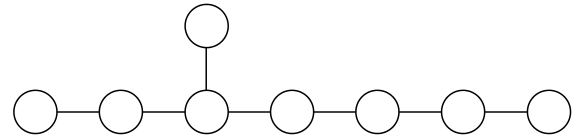
\includegraphics[width=0.6\linewidth]{figures/e8.png}
 \caption{The Dynkin diagram of $E_8$.} 
 \label{e8} 
\end{figure}

To see that $E_8$ is unimodular, we have $\Lambda \supset \Lambda'$ a sublattice with $\det \Lambda' = [\Lambda : \Lambda'] \det \Lambda$. Both $\Z_8$ and $E_8$ contain $D_2$ as an index 2 sublattice, which implies that $\det E_8= \frac{2}{2}\det \Z^8 =1$.


    %\section{J.H.C Whitehead's Theorem on 4-dimensional homotopy types} 
\begin{theorem}
    If $X,X'$ are simply connected, oriented typical 4-manifolds, then any isometry $Q_X \xrightarrow{\cong} Q_X$ of intersection forms comes from an oriented (deg 1) homotopy equivalence $X \to X'$.
\end{theorem}
This comes from a 1949 paper by Whitehead called ``\emph{On simply connected 4-dimensional polyhedra}'', with complications due to $H^3$. For manifolds, $H^3=H=0$, so we get a simpler statement and simpler proof.

\subsection{Overview of relevant homotopy theory}
For a space $X$, call it 0-connected if it's path-connected and for $n\geq 0$, $n$-connected if all based maps $(S^k,*) \to (X,*)$ ($k \leq n$) are based homotopies to constants. In other words, $\pi_k(X,*)=[S^k, X] = 0$ for all $k \leq n$.
\begin{namedthm}{Hurewicz Theorem} 
    Consider the Hurewicz map $h_n  \colon \pi_n (X) \to H_n (X), [\gamma ] \mapsto  \gamma ^*[S^n ]$. If $X $ is $(n-1)$-connected (where $n-1 \geq 1$), then $h_n $ is an \textbf{isomorphism}.
\end{namedthm}
It is often useful to think of the homotopy groups as $\pi_n (X,*) = [(I^n , \partial I^n ),(X,x)]$, since $S^n  = I^n  /\partial I^n $. In other words, we map the boundary of the $n$-cube to the basepoint. Using this picture, composition is easy to draw. There is a relative version of this setup; for $A \subseteq X$, we have a relative homology group $H_*(X,A)$ and a long exact sequence \[
    H_k(A) \to H_k(X) \to H_k(X,A) \xrightarrow{\partial }  H_{k-1}(A)
\] There is something similar for homotopy groups, where $* \subseteq A \subseteq X$. We get relative homotopy groups $\pi_k(X,A)$ sitting in an exact sequence of the same sort: \[
\cdots \to \pi_k(A) \to \pi_k(X) \to \pi_k(X,A) \to \pi_{k-1}(A) \to \cdots 
\] The absolute homotopy gives a small clue of what to do; $I^n $ should map to $X$ while $\partial I^n $ should map to $A$. We have $\pi_n (X,A,*) = \{\text{homotopy classes of maps } (I^n ,\partial I^n ,J^{n-1} ) \to (X,A,*)\} $, where $J^{n-1}:= (\partial I^n ) \setminus \left( \{1\} \times I^{n-1}   \right) $, which is the boundary minus the top face. One can think of $J^{n-1}$ as the ``open'' or lidless cardboard box. Then we have the relative Hurewicz map $\pi_n (X,A,*) \to H_n (X,A)$, which is an isomorphism if $(X,A) $ is $(n-1)$-connected $(n-1 \geq 1)$, or has trivial $\pi_k(X,A) ,\ k \leq n-1$.

\subsection{Whitehead's Theorem}
A map of path-connected spaces $f \colon X \to Y$ is called a \textbf{weak homotopy equivalence} if it induces bijections on $\pi_k(X) \to \pi_k(Y)$ for all $k \in \N$. Some facts:
\begin{itemize}
\setlength\itemsep{-.2em}
    \item If $X,Y$ have the same homotopy type of a CW complex, a weak homotopy equivalence is a homotopy equivalence. 
\item If $X,Y$ are simply connected, and $f \colon X \to Y$ is an $H_*$-isomorphism, then it's a weak homotopy equivalence.
\item If $X$ is a compact smooth manifold, then $X  $ is homotopy equivalent to a finite CW complex.\footnote{Some ways to show this in clude Morse theory which gives a handlebody decomposition, or that X is homotopy equivalent to the nerve of a good covering.}
\item The same is true for $X$ a compact topological manifold (hard).
\end{itemize}
Back to 4 dimensions, let us dicsus the construction of 4-dimensional CW complexes. Start with a wedge sum of $n$ copies of the 2-sphere, $\bigvee^n S^2$. Attach a 4-cell $D^4$ via an attaching map $f \colon \partial D^4 =S^3 \to  \bigvee^n S^2$ which lead to a CW complex $X_f$. This is not yet a 4-manifold and will most likely not be. These spaces tend to be model homotopy types for 4-manifolds. The homotopy type of $X_f$ depends only on the homotopy class of $f$. We can asssume that $f$ respects given basepoints. The main lemma is as follows: 
\begin{lemma}
    We have $\pi^3\left( \bigvee^n S^2 \right) \cong \{n \times n \text{ symmetric matrices over } \Z\} $, where $[f] \mapsto  Q_f$.
\end{lemma}
Note that $H^*(X_f)= \Z_0 \oplus \Z_2^n  \oplus \Z_4$ with basis $e_1,\cdots ,e_n $ of fundamental classes of the 2-spheres. Then $H^2(X_f)=\Hom(H_2(X_f),\Z)\cong \Z^n $ with dual basis $(e^1 ,\cdots ,e^n )$. Now we can write down the matrix $Q_f$. We have \[
    (Q_f)_{ij}= \left\langle \underset{H^4(X_f)}{\underbrace{e^i  \smile e^j }}\, , [X_f]  \right\rangle \in \Z.
\] 
    In the $n=1$ case, we have $\pi_3 (S^2) \underset{\cong }{\xrightarrow{\text{Hopf invariant} }} \Z $.
\begin{proof}[Proof of the case where $n=1$]
    Think of $S^2 = \P^1 \sim \C \mathrm{P^1}\hookrightarrow  \P^2$. We want to know $\pi_3(\P^1)$, which sits inside an exact sequence \[
        \pi_4(\P^2) \to \pi_4(\P^2,\P^1) \to \pi_3(\P^1) \to \pi_3(\P^2)
    \] We have a fibration sequence $S^1  \hookrightarrow S^5\to \P^2$ which is a fiber bundle with fiber $S^1 $. This implies that $\pi_3(\P^2)=0,\pi_4(\P^2)=0$. So $(\P^2,\P^1)$ is 4-connected, and $\pi_4(\P^2,\P^1) \cong H_4(\P^2,\P^1) =\Z$.
\end{proof}
The proof of this key lemma is the generalization of the Hopf invariant.

    %\input{9_14}
    %\input{9_16}
    %\input{9_19}
    \section{Complex structures and self duality, Hodge theory} 
Last time we talked about $n$-dimensional complex vector spaces $V$ with $I = i \cdot  -$ acts on $V$. Then $\Hom _{\R}(V, \C) = V ^{1,0}\oplus V ^{0,1}$ where $I^*=i$ acts on $V ^{1,0}$, and $I^* = -i $ acts on $V^{0,1}$. We then took exterior powers $\bigwedge ^k _{\C}\Hom_{\R}(V,\C) = \bigwedge _{\C}^k \left( V ^{1,0}\oplus V^{0,1} \right)= \bigoplus _{p+q=k}\Lambda ^{p,q} $, where $\Lambda^{p,q}= \mathrm{span}\{a_1 \wedge \cdots \wedge a_p \wedge b_1 \wedge \cdots \wedge b_q \mid a_j  \in V^{1,0}, b_j  \in V^{0,1}\} \cong \Lambda^p V^{1,0}\otimes \Lambda^q V^{0,1}$. Observe that $\Lambda^kI^*$ acts on $\bigwedge ^k _{\C}\Hom _{\R} (V,\C)$ which acts on $i ^{p-q}$ on $\Lambda^{p,q}$.

These are complex forms in some sense, let us say something about real forms. On one hand, one could look at $\bigwedge^k _{\R}\Hom _{\R}(V,\R)$, or the complexification $\bigwedge _{\C}^k \Hom _{\R}(V,\C)$. Canonically we have
\[
    \left( \bigwedge _{\R}^k \Hom _{\R}(V,\R) \right) \otimes \C = \bigwedge _{\C}^k\Hom _{\R}(V,\C)
\] 
which says that passing to exterior powers canonically commutes with extending to scalars. So $\left( \bigwedge _{\R}^k \Hom _{\R}(V,\R) \right) \otimes \C = \bigoplus \Lambda^{p,q}$, e.g. $V = T_x M,\ \left( \Lambda^k T^*_x M \right) \otimes \C = \bigoplus \Lambda^{p,q}$. We understand that $\Lambda^{q,p}= \overline{\Lambda^{p,q}}$ by taking the complex conjugate of $\C$. Then we have real forms $\Lambda^k _{\R}\Hom(V,\R) \subseteq \bigoplus \Lambda^{p,q}$, where $\omega= \sum_{p+q=k} \omega _{p,q}$, $\omega _{q,p}= \overline{\omega _{p,q}}$. 

Let's look at this in complex dimension 2, real dimension 4. In the model case where $V = \C^2$, this has standard basis $\{e_1,e_2\} $, and $V ^{1,0}$ has complex dual $\{e^1,e^2\} $ where $e^j (e_k)= \delta _{jk}$, $e^j $ is $\C$-linear. $V^{0,1}$ then has basis given by the conjugates $\overline{e_1}, \overline{e_2}$ which are $\C$-antilinear. Then we are interested by the 2-forms 
\[
\Lambda^2 \Hom _{\R}(V, \C) = \left( \Lambda^2_{\R}\Hom _{\R}(V,\R) \right)\otimes \C = \underset{e^1 \wedge e^2}{\Lambda^{2,0}} \oplus \underset{e_1 \wedge \overline{e^1}}{\Lambda^{1,1}} \oplus \underset{\overline{e^1}, \overline{e^2}}{\Lambda^{0,2}} 
\]($e_1 \wedge \overline{e^2}, e_2 \wedge \overline{e^1}, e^2\wedge\overline{e^2}$ also lie in $\Lambda^{1,1}$). We can regard $\C^2$ as a real, oriented inner product space with basis $\left( e^1, \overline{e^1}, e^2, \overline{e^2} \right) $. Then $\Lambda^2 _{\R}\C^2= \Lambda^+ \oplus \Lambda^-$, where \[
\Lambda^+ = \left( \Lambda^{2,0} \oplus \Lambda^{0,2}\right) _{\R} \oplus \R(e^1 \wedge \overline{e^1} + e^2 \wedge \overline{e^2}),
\] and
$\Lambda^- = \Lambda^{1,1}_- = \{\eta \in \Lambda^{1,1}\mid  \eta \wedge \omega = 0\} $.
This is a fairly trivial decomposition of 6-dimensional vector spaces; when we bring Hodge theory into the mix, we find that this trivial matter has a highly non-trivial aspect by the Hodge index theorem.

\subsection{Hodge theory}
\begin{namedthing}{Goal} 
    Look at $(H^2(X^4;\R) ,Q_X) \cong  (H^2_{\mathrm{DR}}(X))$  which comes with form $\left( [\alpha ],[\beta ] \right)= \int_X \alpha \wedge \beta  $. These two are canonically identified with a map called ``integration''. Say we have a conformal class of Riemannian metrics $[g]$, which leads to an orthogonal deomposition $H^2_{\mathrm{DR}}(X) = \mathcal H^+ _{[g]}\oplus \mathcal H^- _{[g]}$, so metrics give rise to a positive and negative definite decomposition of cohomology. Specifically, $\mathcal H_g^+$ is the space of  2-forms  $g$ which are self dual and harmonic, while $\mathcal H^- _g$ is the same but anti-self dual.  \textbf{Harmonic forms} are the subject of Hodge theory.
\end{namedthing}

The first part of Hodge theory is something called the \textbf{co-differential}. Here $M^n $ is a manifold, then we have the exterior derivative $d \colon \Omega^k _M \to \Omega^{k+1}_M$. Assume an orientation exists and choose one, plus a Riemannian metric $g$ (a symmetric pairing on each tangent space). We use these to construct the co-differential $d^* \colon \Omega^k \to \Omega^{k-1}$. There are two ways to define this:
\begin{itemize}
\setlength\itemsep{-.2em}
    \item We have the Hodge star $* \colon \bigwedge^k T^*M \to \bigwedge ^{n-k}T^*M$ depending on the metric and the orientation. Then $d^* = \left( -1 \right) ^{k+1}* ^{-1} \circ d \circ *$, where we conjugate the exterior derivative by the Hodge star. This indeed lowers the degree by one. $*$ is nearly an involution, where $* \circ * = \pm \id$. So this is just $\left( -1 \right) ^{k+1}(-1) ^{k(n-k)}* \circ d \circ * =\boxed{  (-1)^{kn+1} * \circ d \circ *}$. Since $d^2=0$, it follows that $\left( d^* \right) ^2 = \pm * d * * d * = \pm * d d * = 0$.
    \item We have an $L^2$ inner product on $k$-forms: $ \langle  \alpha_1, \alpha_2\rangle _{L^2}= \int _M g(\alpha_1,\alpha_2) \mathrm{vol}_g$, where $\alpha_1 \in  \Lambda^k_C$ has compact support, $\alpha_2 \in \Omega^k$. We claim that \[
    \langle d^* \alpha_1, \alpha_2 \rangle _{L^2}= \langle \alpha_1, d\alpha_2 \rangle _{L^2}.
\] This is supposed to be a combination of the construction of the Hodge star with Stokes theorem and integration by parts. That is to say, if we look at $\int_M d(\alpha \wedge \beta )$ where $\deg(\alpha )=k, \deg(\beta )=n-k-1$, $\alpha $ has compact support, Stokes says that this integral is zero. On the other hand,  $\int_M d \alpha \wedge \beta  + (-1)^k \int _M \alpha  \wedge d \beta $ which is integration by parts. This relation plus the definition of the Hodge star implies our claim.
\end{itemize} 
\subsection{Harmonic forms}
Let's bring in harmonic forms now. The Hodge Laplacian $\Delta  = (d+d^*)^2 = d \circ d^* + d ^* \circ d$ is a degree two differential operator $\Lambda^k \to \Lambda^k$. The \textbf{harmonic} $k$\textbf{-forms} are defined as $\mathcal H^K =\ker \Delta $, or the kernel of the Laplacian. Clearly $\ker(d + d^*) \subseteq \mathcal H^k$, but the reverse inclusion holds if $M$ is compact ($\ker(d+d^*) = \mathcal H^k$). Consider a form 
\[
\langle \alpha ,\Delta \alpha  \rangle _{L^2}= \langle \alpha , d^* d \alpha  + dd^* \alpha  \rangle _{L^2}= \langle d^*\alpha , d\alpha  \rangle_{L^2} + \langle d^*\alpha , d^*\alpha  \rangle _{L^2}= \| d\alpha \|_{L^2}^2 + \| d^* \alpha \|_{L^2}.
\] 
This proves the claim, since if the LHS is zero then the two positive terms on the RHS must be zero. Next time we go on with Hodge theory and we will state the Hodge theorem, and combine it with self duality.


    \section{Variational Characterization} 
{\color{red}todo:beginning of this lecture} 
\begin{lemma}
    A harmonic form strictly minimizes $L^2$ norm within its de Rham cohomology class.
\end{lemma}
\begin{proof}
    For $\alpha  \in H_g^k, d\alpha  = 0, d^* \alpha  = 0, \| \alpha \|^2 _{L^2}=\int_M g(\alpha ,\alpha ) \mathrm{vol}_g$. Then 
    \begin{align*}
        \| \alpha  +d \gamma \|^2 &= \langle \alpha  + d\gamma , \alpha  + d \gamma  \rangle _{L^2}\\
                                  &= \| \alpha \|^2_{L^2}+ \|d \gamma \|^2 _{L^2}+ 2 \langle \gamma , d^* \alpha  \rangle _{L^2}\\
                                  &> \| \alpha \|^2 _{L^2}
    \end{align*}for $d\gamma \neq 0$. Conversely, it's easy to check that a  minimizer for an $L^2$ norm in a fixed cohomology class is harmonic. Take some minimizer $\eta$, and look at $\left. \frac{d}{dt} \right| _{t=0}\left( \| \eta  + t d \gamma \|^2 _{L^2} \right) $.
\end{proof}
We are in the world of calculus of variations. Here's the Hodge theorem.
\subsection{The Hodge Theorem}
Note that in $\Omega^k$, we have $\left( \im d^* \right) ^{\perp}= \ker d$. Then $\Omega^k = \ker d \oplus \im d^*$---this would follow formally in a \emph{Hilbert space}, but the $L^2$ norm on $\Omega^k$ is \emph{incomplete}. Nothing is for free.
\begin{namedthm}{Hodge Theorem} 
    We have $L^2$-orthogonal decompositions; $\Omega^k = \ker d \oplus \im d^*,\ \ker d = \mathcal H_g ^k \oplus \im d$ (where $\mathcal H_g^k = \ker d \cap  \ker d^*$. Hence the map  \[
        \mathcal H_g^k \to H_{\mathrm{DR}}^k (M) = \frac{\ker d}{\im d}, \quad \eta \mapsto  [\eta]
    \] is an \textbf{isomorphism}.
\end{namedthm}
At this point in the course we will not go into the proof. Later in the course we will discuss the types of techniques needed to prove this. The proof involves Hilbert space completions of $\Omega^k$ in which the existence of $L^2$ minimizers is a formality. There is something called an ``elliptic regularity'' step to prove that these minimizers lie in $\Omega^k$ and not its completions.

Hodge, being an algebraic geometer, did not think to recruit a collaborator who was an expert in the type of analysis that Hilbert developed. Of course, some mathematicians came in and fixed all the issues later (von Weyl, Kodaira).

\subsection{Hodge theory and self duality}
Now we come to the 4-dimensional case, where we relate Hodge theory to self duality. Let $X^4_g$ be a compact Riemannian (we only need the conformal class of $g$, or $g \sim \lambda g$ for $\lambda \colon x \to (0, \infty) \subseteq \R$) oriented 4-manifold. The codifferential for 2-forms is $d^* = -*d* \colon  \Omega^2 \to \Omega$. For $\eta \in \Omega^2$, $\eta \in \ker (d + d^*)$ or harmonic iff $*\eta \in \ker(d+d^*)$. If $\eta \in \mathcal H^2 _g$, then $\eta ^{\pm}= \frac{1}{2}(\eta \pm *\eta)\in \mathcal H^2_g$. Also, a self-dual 2-form is harmonic iff it's closed. The upshot is that $\mathcal H^2 _g = \mathcal H^+ \oplus \mathcal H^-,$ where $\mathcal H ^{\pm}= \mathcal H^2 \cap \Omega^{\pm}$. In otherwords, $\mathcal H^2_g$ is the sum of the self dual harmonic forms and the anti-self dual harmonic forms. OTOH, we have $\mathcal H^2 \xrightarrow{\cong } H _{\mathrm{DR}}^2 (X)$ by the Hodge theorem.
If $\omega \in \mathcal H^+$, then \[
    \int_X \omega \frown \omega = \int (\omega * \omega) \smile 0) = \int |\omega|^2 \mathrm{vol} >0.
\] If $\omega \in \mathcal H^-$, then \[
\int \omega \wedge \omega = -\int |\omega|^2 \mathrm{vol}<0.
\] We have the second Betti number $b^2(X)= b^+ + b^-$, and $\tau(X) = b^+ - B^-$, where $b^{\pm}=\dim \mathcal H^{\pm}$.

\subsection{The self-duality complex}
Perhaps this is the title of one of the lesser known paper of Sigmund Freud. We are still on $(X^4, g)$ our compact, oriented 4-dimensional Riemannian manifold. We examine the cochain complexes 
\[
0 \to \Omega^0 \xrightarrow d\Omega^1 \xrightarrow{d^+} \Omega^+ \to 0
\] as follows. Consider $d^+ \alpha  = (d\alpha )^+ = \frac{1}{2}(1 +*)d\alpha $ as a cochain complex $\left( \mathcal E^*, \delta \right) $. The result we want to explain is the following.
\begin{theorem}
    The cohomology of $\mathcal E^*$ is 
    \begin{align*}
        H^0(\mathcal E) &= H^0 _{\mathrm{DR}}(X)\\
        H^1(\mathcal E) &\cong  H^1 _{\mathrm{DR}}(X)\\
        H^2(\mathcal E) &\cong \mathcal H^+ _g.
    \end{align*}
\end{theorem}
This is the prototype of things that come up in gauge theory a lot, specifically one often looks at 1-forms simultaneously in the kernel of $d^+$ and the codifferential adjoint of $d$.
\begin{proof}
    It is easy to check the $H^0$ case. For $\alpha  \in \Omega^1$, we have $d\alpha  + d^+ \alpha  + d^- \alpha $, so \[
        \int_X d\alpha  \wedge d\alpha  = \| d^+ \alpha \|^2_{L^2}- \| d^- \alpha \|^2 = \int_X d(\alpha  \frown d\alpha ) \underset{\text{Stokes}}{=} 0.
    \]  So $\| d^+ \alpha \|_{L^2}= \| d^- \alpha \|_{L^2}$, and $\ker d^+ = \ker d^- = \ker d$. Hence $H^1(\mathcal E) \to H^1 _{\mathrm{DR}}(X), \ [\alpha ]\mapsto  [\alpha ]$ is an isomorphism.

    We want $\mathcal H^+_g$ identified with $\omega \in \frac{\Omega^+}{\im d}$. Then $\omega = \omega _{\text{harm} }+ d\alpha  + * d\eta$, OTOH $*\omega = \omega$ since we assumed it to be self dual. Then $d\alpha  + *d \eta = 2d^+ \alpha $.
\end{proof}



    \section{The period map and the integer lattice} 
Last time we talked about how a choice of metric gives a splitting of the second de Rham cohomology. This week we look more closely at this splitting and how it interacts with the integer lattice within that second de Rham cohomology. There will be some differential geometry and a bit of analysis this week.

For any smooth manifold $M^n $ and any $k \in \Z _{\geq 0}$, there is an additive subgroup $H_{\Z}^k \subseteq H^k  _{\mathrm{DR}}\left( M \right) $ of ``integer classes'', i.e., classes $[\alpha ]$ of closed  $k$-forms $\alpha $ with \textbf{integer periods}; $\int_P \alpha  \in \Z$, for all smooth singular $k$-cycles $P$ (smooth compact oriented $k$-dimensional manifolds). This subgroup is a \textbf{lattice}, a 4-dimensional discrete subgroup, or the inclusion extends to an $\R$-linear isomorphism, and extending the coefficients to $\R$ is an isomorphism; $H_{\Z}^k \otimes \R \xrightarrow{\cong } H^k_{\mathrm{DR}}(M)$.
Why is this a lattice?  \[
    H^k_{\mathrm{DR}}\left( M \right) \cong  H^k(M; \R) \underset{\text{universal coefficients}}{\cong}  H^k(M;\Z)\otimes \R = H^k(M;\Z)'=\frac{H^k(M;\Z)}{\text{tors}} \otimes \R.
\] Then $H^k(M;\Z)' \hookrightarrow H_{\mathrm{DR}}^k(M)$ maps isomorphically onto $H_{\Z}^k$. Call the subgroup $H^k _{\Z}$ the \textbf{integer lattice}.

\subsection{The 4-dimensional case}
For $X^4$ closed and oriented, we have our quadratic form on $H^2_{\mathrm{DR}}(X)$, where $\eta \mapsto  \int_X \eta \wedge \eta$. From last time, we saw using Hodge theory that $H^2_{\mathrm{DR}}(X)=\mathcal H^+_{[g]} \oplus \mathcal H^-_{[g]}$, where these subspaces depend on a choice of conformal structure. Then $\mathcal H^{\pm}_{[g]}(\Z) := H^2 _{\Z}\cap  \mathcal H^{\pm}_{[g]}$.
Recall that $b^+ = \dim \mathcal H^+, b^- = \dim \mathcal H^-$. 
\begin{theorem}
    Assume $b^+(X) > 0$. Then for generic conformal structures $[g]$, we have $\mathcal H_{\Z}^- =0$. 
\end{theorem}
Precisely, we work with conformal classes of $C^r$ Riemannian metrics, $r \in \N, r \geq 3$. ``Generic'' means it holds on a countable intersection of open dense subsets. It turns out spaces $\mathcal C_r(X)$ of conformal structures identified with an open ball in a Banach space.
\begin{cor}
    $\mathcal H_{\Z}^- = 0$ for a \textbf{dense} set of $C'$ conformal structures.
\end{cor}
\begin{proof}
    Apply the Baire category theorem in the closure of the open ball. 
\end{proof}

\subsection{The period map}
This is a map $P \colon \mathcal G_r(X) \to \mathrm{Gr}^-, \ [g] \mapsto  \mathcal H^- _{[g]} \subseteq H^2s_{\mathrm{DR}}(X)$, where $\mathrm{Gr}^-$ is short for $\mathrm{Gr}^-_{b_-}\left(H^2 _{\mathrm{DR}}(X)\right)$, the Grassmannian of $b_-(X)$-dimensional subspaces of $H^2_{\mathrm{DR}}(X)$. The minus means we want the subspace to be negative definite for the quadratic form. The proof will involve $P$ and its derivative.
We've taken calculus and know how to differentiate things. How do we differentiate the period map?

The simplest part of the story, yet the most instructive and important, has to do with the Grassmannian itself. The Grassmannian $\mathrm{Gr}^-$ has submanifolds $S_{c}$ for any $0\neq c \in H^2_{\mathrm{DR}}(X)$, where $S_c := \{J \in \mathrm{Gr}^- \mid c \in J\}$.

\begin{figure}[H]
\centering
 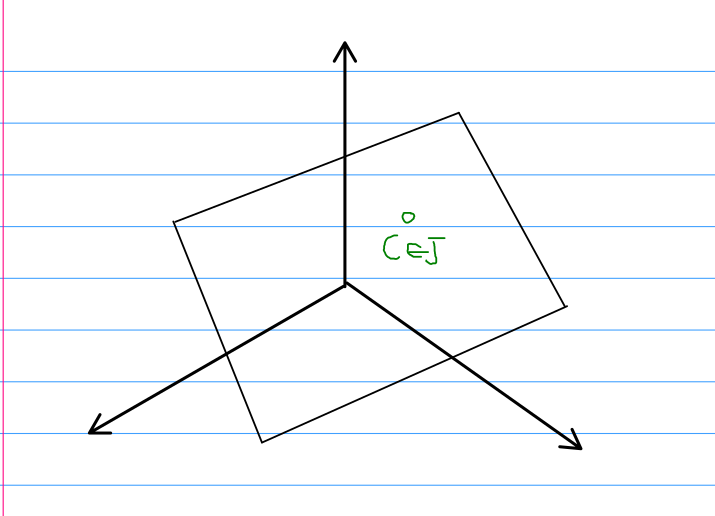
\includegraphics[width=0.3\linewidth]{figures/grass.png}
\caption{Visualizing some $J \in S_c$.}
\label{grass}
\end{figure}
Why is $S_c$ a submanifold? Consider charts on $\mathrm{Gr}$ (or $\mathrm{Gr}^-$). For $J \in \mathrm{Gr}$, choose a complement $K$, so $H = J \oplus K = H^2 _{\mathrm{DR}}(X)$. Then $\Hom _{\R}(J,K) \xrightarrow{\phi _{J,K}} \mathrm{Gr}, \theta \mapsto  \mathrm{graph}(\theta)$, where $\phi _{J,K}$ is an atlas for $\mathrm{Gr}$. Suppose now that $c \in J$, or $J \subseteq S_c$. $\phi _{J,K}$ maps $\{\theta \in \Hom(J,K) \mid \theta(c) = 0\} $ to a neighborhood of $J$ in $S_c$, i.e. we get a \emph{submanifold} chart. Since $b^+ > 0$, $\mathrm{Gr}^- \setminus S_c$ is open and dense in $\mathrm{Gr}^-$. We can look at $\bigcup_{0\neq c \in H^2_{\Z}} S_c \subseteq \mathrm{Gr}^-$, a countable union of closed submanifolds of positive codimension, and is \emph{generic}  (no idemp sets). What this tells us is that our intution that if we look at a Grassmannian and a random subspace to see how it intersects the integer lattice is that it only intersects at the origin. 

Our next step is to show that $P$ is transverse to each of the submanifolds $S_c$ where $0\neq c \in H^2_{\Z}$. This implies that $P^{-1}(S_c) \subseteq \mathcal C_r(X)$ is a closed codimensional $b^+$ submanifold (where $\mathcal C_r(X)$ is an $\infty$-dimensional manifold). This implies our theorem. Transversality means that if $P[g] \in S_c$, then $\boxed{T _{P[g]}^{\mathrm{Gr}^-}= T_{P[g]}S_c + \im D_{[g]}P}$ (the derivative of the period map). This is the technical statement that is going to be proved. Some of the proof will be next time, primarily using a Hodge theoretic calculation. First you differentiate the Hodge star with respect to the conformal structure, then you differentiate the period map. It also uses a principle from PDEs, called unique continuation for harmonic 2-forms.


    \section{The period map and the integer lattice, continued} 
Let $X^4$ be a closed, oriented manifold, and $P \colon \mathcal C(X) \to \mathrm{Gr}^- \subseteq \mathrm{Gr}_{b^-(X)}(H^2_{\mathrm{DR}}(X))$, where $\mathcal C(X)$ is the set of conformal structures. Then $P[g] = \mathcal H^- _{[g]}= \{g\text{-ASD harmonic functions} \} $. So $\mathcal H_{[g]}^- (\Z) = \mathcal H^-_{[g]} \cap  H^2(X,\Z) \subseteq H^2 _{\mathrm{DR}}(X) = P[g] \cap H^2(X,\Z)$. The generic non-existence theorem says that for generic $[g], b^+ >0$, we have  $\mathcal H ^- _{[g]}(\Z) = 0$.
For $S_c \subseteq \mathrm{Gr}^- $ (submanifolds of codimension $b^+$), the claim is that $P \transv c$ for each $c$. Hence $P^{-1}(S_c)$ is a codimension $b^+$ submanifold of $\mathcal C(X)$.
The theorem holds since generic conformal structures don't lie in the countable union $\bigcup_{c} P^{-1}(S_c)$.

\begin{remark}
    In families of conformal structures, $\mathcal H _{[g]}^- (\Z) \neq 0$ occurs with codimension $b^+$ in the parameter space.
\end{remark}
We need to understand the manifold structure of $\mathcal C(X)$. 

\subsection{Conformal structures as maps $\Lambda ^- \to \Lambda^+$}
Let $V$ be a 4-dimensional oriented vector space. Choose a reference inner product $g_0$, which gives rise to a splitting $\Lambda^2V = \Lambda_0^+ \oplus \Lambda_0^-$. If $\Lambda^-$ is another 3-dimensional subspace of $\Lambda^2V$ that is negative definite with respect to the squaring form $\eta \mapsto \eta \wedge \eta$, then the projection $\Lambda^- \xrightarrow{\cong} \Lambda_0^-$ is an isomorphism. So $\Lambda^- = \Gamma_ m = \mathrm{graph}\left(m \colon \Lambda_0^-  \to \Lambda_0^+\right)$, where $ m \subseteq \Hom(\Lambda_0^-, \Lambda_0^+)$.

We could ask which linear maps $m$ give rise to a negative definite subspace. For $m \in \Hom (\Lambda_0^-, \Lambda_0^+)$, $\Gamma_m$ is negative definite iff $|m| _{\mathrm{op}}<1$. Then $g(\eta) = \eta ^2$, and 
\[
    g(\alpha  + m\alpha  ) = g(\alpha ) + g(m\alpha ) = \underset{<0}{\underbrace{\left( -|\alpha |^2 + |m\alpha |^2 \right)}}  \mathrm{vol}.
\] 
\begin{prop}
    The map $m \mapsto \Gamma_m$ identifies linear maps $\Lambda_0^- \to \Lambda_0^+$ of operation norm $<1$, with negative definite 3-dimensional subspaces of $\Lambda^2V$. Then conformal structures are in bijection with the set $\left\{m \,\big|\, |m| < 1\right\} $.
\end{prop}
This tells us that conformal structures are not identified by some complicated manifold, but just some ball in a vector space.
\begin{remark}
    If $\Lambda^- = \Gamma_m$, then $\Lambda^+ = (\Lambda^-) ^+ = \gamma _{m^*}$, where $m^*$ is adjoint to $m$.
\end{remark}
This is the linear algebra picture, the globalization is essentially immediate. The conformal structures on our 4-manifold are identified with vector bundle maps $\Lambda_{g_0} ^- \xrightarrow{m}  \Lambda_{g_0} ^+$ with reference metric $g_0$, with the property that $|m_x| _{\mathrm{op}}<1$ for all $x \in X$. Here $X$ is compact, and $c \mapsto  C^r$ is a bundle map, an open subset of a Banach space.

We compute that \[
    D_{[g_0]}P \colon T_{[g_0]}\mathcal C(X) \to  T_{P[g_0]}\mathrm{Gr}^- = C^r(X, \Hom(\Lambda_{g_0}^-, \Lambda_{g_0}^+)) \to \Hom (\mathcal H^-, \mathcal H^+).
\] 
\begin{prop}
    For $m$ a bundle map, $\alpha ^- \in \mathcal H^-$, \[
        (D_{[g_0]}P)(m) (\alpha ^-) = m(\alpha ^-)_{\mathrm{harm} } \in \mathcal H^+.
    \] So this is a harmonic orthogonal projection $\Omega_{g_0}^+ = \mathcal H^+ \oplus \im d^+\to \mathcal H^+$ (conformal self-duality complex).
\end{prop}
This is the claimed answer, and it is as clean as can be. In differential topology, often you are faced with scary tasks like differentiating a map between complex structures. If you can unravel to the point where you can really formulate what you need, it is more feasible to guess what the answer should be and go from there.

We use this to show that $P\transv S_c$, i.e., $T_{P[g]}\mathrm{Gr}^- = T_{P[g]}S_c + \im D_{[g]}P$. We need that $\im DP$ spans the normal space $T_{P_{g_0}}\mathrm{Gr}^- / T_{p_g}S_c = N_{P_g}(S_c)$. We have \[
    N_J S_c = \frac{T_J \mathrm{Gr}^-}{T_J S_c} = \frac{\Hom (J,J^{\perp})}{\{\theta \in \Hom(J, J^{\perp}) \mid  J(c) = 0\} \underset{\theta \mapsto  \theta(c)}{\xrightarrow{\cong}}  J^{\perp}}.
\] Unraveling this lot, we find out that what we need to prove is the following:
\begin{itemize}
\setlength\itemsep{-.2em}
    \item If $\alpha  ^- \in \mathcal H^-_g$ represents $0\neq c \in H^2(X,\Z)$, then for all $\alpha  ^+ \in \mathcal H^+_g,$ there exists a bundle map $m \colon \Lambda_g^- \to \Lambda_g^+$ with the property that $m(\alpha ^-) _{\mathrm{harm}} = \alpha ^+$.
\end{itemize}
If not, then there exist forms $\alpha ^{\pm}\in \mathcal H ^{\pm}_g$ such that $\alpha ^+ \perp _{L^2}m(\alpha ^-)_{\mathrm{harm}}$ for all $m$. So $0 = \langle \alpha ^+, m(\alpha ^-) _{\mathrm{harm}} \rangle _{L^2} = \langle \alpha ^+, m(\alpha ^-) \rangle _{L^2}$ for all $m$. For such a vanishing to hold for all bundle maps $m$ seems very strong. Say there exists an $x \in X$ where $\alpha _x^+ \neq 0, \alpha _x^- \neq 0$. Use bundle maps $m$ supported by $x$ to get a contradiction. We conclude that either $\alpha ^+ $ or $\alpha ^-$ must be identically zero on some open set. There is a unique continuation principle that says a harmonic form vanishing to infinite order of a point vanishes everywhere. Hence $\alpha ^- = 0$ or $\alpha ^+ =0$ implies they both are zero, or $\alpha ^+ = \alpha ^- = 0$. 

Next time, complex geometry.

    \section{Hodge Theory on complex surfaces} 
Today we will discuss the Hodge index theorem and KS surfaces.
\subsection{K\"ahler manifolds}
Let $X$ be a complex manifold (holomorphic atlas), and $J$ be a complex structure, where $J \colon TX \to TX$, $J = i \cdot -$. Then we have the \textbf{hermitian metric} on $X:$ \[
h_x \colon T_x X \times T_x X \to \C
\] for all $x \in X$.\footnote{Something about this is different from the quantum mechanical definition.} It satisfies the following properties:
\begin{itemize}
\setlength\itemsep{-.2em}
    \item It is $\R$-bilinear,
    \item $h_x(Ju,v) = ih_x(u,v) = -h_x(u,Jv)$,
    \item $h_x(v,n) =  \overline{h_x(v,v)}$,
    \item $h_x(u,u \in \R) > 0$ for every $u \neq 0$.
\end{itemize}Then $h = g+ i\omega$, where $g$ is a Riemannian metric for $J \in O(g)$, and $\omega$ is a 2-form, where $\omega (J_n ,J_v) =  \omega(u,v)$. Think of $J$ as given. Then $\omega \leftrightarrow g$, with $g(u,v) =\omega (u, Jv)$, etc. So $\Lambda^2(X) \otimes \C = \Lambda^{2,0}\oplus \Lambda_{1,1}\otimes \alpha ^{0,2}$, with eigenvalues $i^2,i^0, i ^{-2}$, since this is $i ^{p-q}$ on $\Lambda^{p-q}$. This distinguishes $\omega$ as a $(1,1)$-form since it lives in the right eigenvalue of $J$. 
We can think of $h$ as determining and being determined by this $(1,1)$-form $\omega$, such that $\omega(v, Jv)>0$ for all $v\neq 0$.
\begin{definition}[]
    A \textbf{K\"ahler manifold} $(X,J,h = g+i \omega)$ is a complex manifold plus a hermitian metric $h$ such that $d\omega =0$. In other words, its imaginary part $\omega$ is a closed 2-form.    
\end{definition}
This is a mysterious yet natural condition, since 2-forms being closed is something to think about. Instead of $h$, you can specify a closed positive $(1,1)$-form $\omega$ (positive means $\omega(v,Jv) >0$). Here $g$ is called a \textbf{K\"ahler metric} and $\omega$ is called a \textbf{K\"ahler form}. So K\"ahler forms are the harmonious intersection between complex, symplectic, and Riemannian geometry.
\begin{example}
    Some examples:
    \begin{itemize}
    \setlength\itemsep{-.2em}
        \item For the complex tori $T = \C^n  /$lattice, it has a complex structure and $\omega$ an intersection form on $\C^n $, which is translation invariant.
        \item  A crucial example is $\C \mathrm{P^N }$. The assertion is that this carries a unique K\"ahler form $\omega_{\C \mathrm{P^N }}$ such that it is as symmetric as can be, that is, $\omega _{\C\mathrm{P^N}}$ is invariant under the action of $PU(N+1)$ on $\C \mathrm{P^N}$. So $\int _{\C \mathrm{P^1}}\omega _{\C\mathrm{P^N}}=1$. We will see this form often as the curvature of a line bundle. In general we have a K\"ahler class $[\omega] \in H^2_{\mathrm{DR}}(X)$, but in this case $[\omega _{\C \mathrm{P^N}}]$ actually lies in the integer lattice $H^2_{\Z}$.
        \item If $X \subseteq \C \mathrm{P^N}$ is a complex submanifold, then the restriction $\left. \omega _{\C \mathrm{P^N}} \right| _X$ is a K\"ahler form. Then smooth algebraic varieties (things cut out of $\C \mathrm{P^N}$ with homogeneous equations) admit K\"ahler forms, moreover \emph{integral} K\"ahler forms ($[\omega] \in H^2_{\Z}$).
            \item The \textbf{Kodaira embedding theorem} says that if $X$ a complex complex manifold admits an integral K\"ahler form, then $X$ embeds in $\C \mathrm{P^N}$ for sufficiently large $N$. For example, integral K\"ahler forms are extremely cheap for Riemann surfaces; take any volume form with integral one. Then by Kodaira's theorem this embeds in complex projective space.
            \item \textbf{Chow's theorem} says that $X$ is furthermore algebraic. So the Riemann surface is actually cut out by homogeneous polynomial equations.
    \end{itemize}
\end{example}

\subsection{Hodge theory}
We will only make assertions here, no proofs. For $(X,J, h = g+ i\omega)$ a compact K\"ahler manifold, the $(p,q)$-components of a $g$-harmonic $k$-form are still harmonic. The differential forms split up as $\Omega^k \otimes \C = \bigoplus_{p+q=k} \Lambda^{p,q}$. It turns out that the \emph{harmonic} $k$-forms split up the same way; $\mathcal H^k \otimes \C = \bigoplus _{p+q=k}\mathcal H^{p,q}$,  where $\mathcal H ^{p,q}$ is $\Lambda ^{p,q}\cap (\mathcal H^k\otimes \C)$. This turns out to be \emph{extremely} useful.

Recall that $\overline{\Lambda^{p,q}}= \Lambda^{q,p}$. So $\mathcal H ^{p-q}= \mathcal H ^{q,p}$. We have $h ^{p,q}= \dim \mathcal H ^{p,q}$, so the Betti number is given by $b^k = \sum _{p+q=k}h ^{p,q}$, where $h ^{qp}= h ^{pq}$.
\begin{definition}[]
    A \textbf{Hodge structure} of weight $k$ on an abelian group $H _{\Z}$ is a vector space decomposition \[
    H _{\Z}\otimes \C = \bigoplus _{p+q=k}H ^{p,q}, \quad H ^{q,p}=\overline{ H ^{p,q}}.
    \] 
\end{definition}
For $X$ compact K\"ahler, we get a weight $k$ Hodge structure on $H^k(X;\Z)$, because
\[
H^k (X;\Z)\otimes \Z \cong \mathcal H^k \otimes \C = \bigoplus \mathcal H ^{p,q}.
\] Note that this is is a similar flavor to the things we've been talking about our Riemannian 4-manifolds, with the decomposition into the self dual and anti-self dual parts. The word ``period map'' is really borrowed from Hodge theory. 
Even more is true. The space $\mathcal H ^{p,q}$ is canonically identified with a gadget form complex analytic geometry, the $q$-th \emph{sheaf cohomology} $H^q(X;\mathcal A^p)$, where  $\mathcal A^p  = \Lambda_{\mathcal O_X}^p(J^*X)$ is the $p$-th exterior power of the holomorphic cotangent sheaf, and $\mathcal O_X$ is the sheaf of holomorphic functions. For example, if $X$ is a compact Riemann surface, \[
    \underset{\dim 2g}{\underbrace{H^1(X, \C)}}  = \underset{g, \text{ holomorphic 1-forms}}{\underbrace{H^0(J^*X)}}  \oplus \underset{g}{\underbrace{H^1(\mathcal O_X)}} 
\] We cannot say much about $H^1$ and $H^2$, but $H^0(\mathcal A^p)$ is the set of holomorphic $p$-forms, which is locally (on $(z_1, \cdots ,z_n )$) the sum $\sum _{|I| = p}f_I dz_I$ for $f_I$ holomorphic.

\subsection{Complex K\"ahler surfaces}
We have $H^2 (X;\C ) = \mathcal H ^{2,0}\cong  H^0(\mathcal A^2)\oplus \mathcal H ^{1,1}\cong  H^1(\mathcal A^1) \oplus \mathcal H^{0,2}\cong  H^2 (\mathcal O)$, where $\mathcal H^{2,0}\leftrightarrow \mathcal H^{0,2}$ and $\mathcal H^{1,1}\leftrightarrow \mathcal H^{1,1}$ by complex conjugation. We saw (pointwise) that $\Lambda^2 \otimes \C = \Lambda^+ \otimes \C \oplus \Lambda^- \otimes \C$. We observed that $\Lambda^+ \otimes \C = \Lambda^{2,0}\otimes \C \cdot \omega \oplus \Lambda^{0,2}$, and $\Lambda^- \otimes \C = \Lambda^{1,1}_0$ for $\omega ^{\perp}$. What we can do is apply this \emph{globally} to harmonic 2-forms; what we get is that self-dual harmonic forms complexified consist of the the harmonic $(2,0)$ forms, harmonic $(0,2)$ forms, and complex copies of the K\"ahler form $\omega$. \[
\mathcal H^+ \otimes \C = \mathcal H ^{2,0}\otimes \C \cdot  \omega \oplus \mathcal H ^{0,2},
\] where $\mathcal H^- = \mathcal H ^{1,1}_0$ for $\omega ^+ \subseteq \mathcal H ^{1,1}$. This just follows from the pointwise calculation we just did. This immediately implies what we call the Hodge index theorem.
\begin{namedthm}{Hodge index theorem} 
   For $X$ a compact K\"ahler surface, 
   \begin{itemize}
   \setlength\itemsep{-.2em}
       \item $b^+ = 1 + 2 h ^{2,0}$. 
       \item Moreover, the wedge product form on $\mathcal H^{1,1}, \eta \mapsto  \int _X \eta \wedge \eta$ has ``signature'' $(1, b^- -1)$.
   \end{itemize}
\end{namedthm}
For example, if you look at the N\'eron-Severi group $\mathrm{NS}(X) = \mathcal H ^{1,1} \cap  H^2_{\Z}$, it has a complex curve $C \subseteq X$, and $PD[C] \in  \mathrm{NS}(X)$. So the intersection form on $\mathrm{NS}(X)$ is negative definite on $\perp $ to $[\omega]$.


    \section{$K 3$ surfaces and periods} 
New topic: covariant derivatives, curvature, and gauge transformations.
\subsection{$K 3$ surfaces}
\begin{definition}[]
    A $K3$ \textbf{surface}  $(X,J)$ is a compact complex surface with $b^1(X) = 0$ with admits:
    \begin{itemize}
    \setlength\itemsep{-.2em}
        \item a K\"ahler structure $g+i\omega$
        \item a nowhere vanishing holomorphic 2-form $\sigma$
    \end{itemize} i.e., has local holomorphic coordinates $(z_1,z_2)$, $\sigma = h(z_1,z_2)dz_1 \wedge dz_2$ where $h$ is holomorphic and non-zero.
\end{definition}
Any \emph{other} holomorphic 2-form $\sigma'$ is $\sigma' =f \sigma$, where $f$ is holomorphic on $X$. The maximum modulus theorem then implies that $f$ is constant, so $H^0(\mathcal A^2)$ (global holomorphic 2-forms) is $\C \sigma$ which implies $h ^{20}=\dim H^0(\mathcal A^2) = \dim \mathcal H ^{20}=1$, since $h ^{02}= h ^{20}=1$ and $\mathcal H ^{02}= \overline{\mathcal H ^{20}}$.
Last time we ended with the Hodge index theorem, which says that for a H\"ahler surface (compact), $b^+ = 1 + h ^{02} + h ^{20}=3$. So $b^+(K 3) = 3$. Moreover we get that the self dual harmonic forms $\mathcal H ^+ _g$ are spanned by the real part of  $\C\sigma\oplus\C \overline{\sigma}\oplus \R \omega$ (where elements of $\C \overline{\sigma}$ look like $a\alpha +\overline{a}\overline{\sigma}$ for $a \in \C$).

There is a magic formula, a version of the Riemann-Roch theorem which says that \[
    \sum (-1)^q h ^{0,q}= \frac{1}{12}\left( c_1^2 (TX)+ c_2(TX) \right) [X]
\] leading to a beautiful characterisation of the Euler characteristic, where $\chi(X) = c_2(TX)[X] = 24$. Here $b^1=0$ by assumption, so $\chi(X) = 2+ b^2$. This implies that $b^2 = 22$, $b^+ = 3$, and so $b^-= 19$. Then you have a Hodge structure $H^2(X) \otimes \C = \mathcal H ^{20}\oplus \mathcal H ^{11}\oplus \mathcal H ^{02}$. Knowing $\C \sigma$, we get $\mathcal H ^{20}= \C \sigma$, $\mathcal H ^{02}=\overline{\C \sigma}$, and $\mathcal H ^{11}= \left( \C \sigma \oplus \C \overline{\sigma} \right) ^{\perp}$, where $[\eta] \in H^2 _{\mathrm{DR}}(X,\C)$, and $\int_X\eta \wedge \sigma =\int_X \eta \wedge \overline{\sigma}=0$. Here $\C\sigma$ is by the Hodge theorem; note that $\int \sigma \wedge \sigma = 0,$ while $\int \sigma \wedge \overline{\sigma}>0$. 
We can record the Hodge structure of a $K 3$ surface $(X,J)$ as its \textbf{period point} $\C \sigma$ in the \textbf{period domain} \[
    P = \left\{ \C \sigma \in \mathbb P (H^2(X,\C) )\,\Big|\,  \int \sigma \wedge \sigma = 0, \int \sigma \wedge \overline{\sigma}>0 \right\} 
\] This is a 20-dimensional complex manifold; $H^2(X,\C)$ is 22 dimensional, projection takes this down to 21 dimensions, the quadratic equation $\sigma \wedge \sigma$ takes this down to 20 dimensions, and $\sigma \wedge \overline{\sigma}$ is an open condition. This is equivalent to the Hodge structure. It is a fact that all points of $P$ occur as period points. It is not quite true that the period point determines the $K 3$ structure up to isomorphism, but ``nearly''.
Some $K 3$ surfaces are ``algebraic'', i.e. there exists a K\"ahler class $[\omega] \in H^2\Z$. For example:
\begin{itemize}
\setlength\itemsep{-.2em}
    \item quartic surfaces in $\C \mathrm{P^3}$
    \item quadric and cubic in $\C \mathrm{P^4}$
    \item double cover of $\C \mathrm{P^2}$
    \item  branched along a smooth sextic curve
\end{itemize}
This takes the dimension down to 19. We briefly mentioned the N\'eron-Severi group $\mathrm{NS}(X,J) = H ^{11}\cap H^2_{\Z}$, the classes of complex curves on $X$. Then $\rho(X) = rk \mathrm{NS}$, the ``Picard point'', and $\rho \geq 1$ for $X$ algebraic. Having $\rho$ \emph{big} is \emph{special}, e.g. for a \emph{generic} quartic surface, $\rho = 1$. This ends our sketchy overview of $K 3$ surfaces.

\subsection{Connections and vector bundles}
We move toward Gauge theory proper. To set a convention, let $E \to X$ be a smooth complex vector bundle, with a Hermitian inner product $h $ in $E$.

\begin{definition}[]
    A \textbf{covariant derivative} (also known as a \textbf{connection}) $\nabla \in E$ is a $\C$-linear map $\nabla \colon C^{\infty} (X,E)\to C ^{\infty}(X, T^*X \otimes _{\R}E) $ from the space of sections to the sections of the cotangent bundle tensored with $E$. It has the property that for a $C ^{\infty}$ function $f$ and section $s$, we want to the Liebniz rule to hold in a sense, or \[
        \nabla  (fs) = df \otimes s + f \nabla s
    \] where $df$ is the exterior derivative of $f$ (a 1-form). It is called \textbf{unitary} (with respect to a Hermitian inner product $h$) if \[
    d(h(s_1,s_2)) = h (\nabla s_1,s_2) + h(s_1, \nabla s_2).
    \] In other words, we want the connection to obey some form of the product rule.
\end{definition}

For any vector field $V \in C ^{\infty}(X,TX)$, we get $\nabla_V \colon C ^{\infty}(X,E) \to C ^{\infty}(X,E)$; for $\nabla_V s$, contract $X$ into $\nabla s$. It is a quick and easy check that $\nabla$ is a \emph{local operator}, that is to say, $(\nabla s)(x)$ depends only on the germ of $s$ near $x$ (in fact this is a weaker statement, it only depends on the first order of the germ of $s$). 

\begin{example}
In the trivial line bundle $\C$, the projection $X \times \C \to \C$, a section of the covariant derivative amounts to a $\C$-linear map $\nabla \colon C ^{\infty} (X,\C)\to C ^{\infty}(T ^* X \otimes \C)$ obeying the Liebniz rule. For example, the exterior derivative $d$ does the job, called the trivial covariant derivative. If we use the obvious Hermitian metric on $\C$ (given by the standard Hermitian metric of $\C$ independent of where you are on $X$), then $d$ is unital. This is essentially the product rule. 
    

    If $V$ is a complex vector space, we get a trivial vector bundle $V = V \times X \to X$, which carries a trivial connection as well; $d_V = d \otimes \id _V$.
\end{example}
The difference $\nabla - \nabla '$ between two covariant derivatives $E \to X$ has the property of being linear over functions($C ^{\infty}(X)$-linear), or 
\begin{align*}
    \nabla (fs ) &= df \otimes s  + f \nabla s\\
    \nabla' (fs ) &= df \otimes s  + f \nabla' s 
\end{align*} Taking the difference will result in something linear over functions. So $(\nabla-  \nabla')s = \alpha s$, where $\alpha _x \in \mathrm{End}_{\C}(E_x)$. What we find is that given a covariant derivative $\nabla$ in $E$, the space of covariant derivatives is given by $\nabla$ plus the vector bundle consisting of the cotangent bundle tensored with endormorphisms of $E$
, or \[
    \{ \text{covariant derivatives in } E\} = \nabla + C ^{\infty}\left(X, T^*X\otimes _{\R}\mathrm{End}_{\C}E\right)
\] The space of covariant derivatives is an affine vector space modelled on the vector space of 1-forms valued in $\mathrm{End}(E)$. In some sense they are pretty straightforward objects. We will continue with this on Wednesday.

    \section{Gauge transformations, curvature, and characteristic classes} 
\subsection{Gauge transformations}
Let $E \to M$ be a complex vector bundle. A \textbf{gauge transformation} is an automorphism $ u \colon E \xrightarrow{\cong } E $, which form a group $G_E$. There is a bundle (\emph{not} a principle bundle) of Lie groups \[
\begin{tikzcd}
\mathrm{GL}(E) \arrow[rr, phantom] \arrow[rd] & \subset & \mathrm{End}_{\C}E \arrow[ld] \\
                                              & M       &                              
\end{tikzcd}
\] with $G_E$ the group of sections of $\mathrm{GL}(E) \to M$. When a hermitian metric in $E$ is given, consider the \textbf{unitary} gauge transformations (sections of $U(E) \to M$). If $u \colon E \to E'$ is a vector bundle isomorphism, a covariant derivative $\nabla$ in $E$ induces $\Delta '$ in $E'$. Then \[
\Delta '_v = u \circ \nabla_v \circ  u^{-1}
\] for all vector fields $v$. So $G_E$ acts on the left on $\mathcal{C} _E = \{\text{covariant derivatives in } E\} $, and \[
u \cdot \nabla = u \circ \nabla \circ u^{-1}.
\] Some cultural confusion; in physics (QFT), they will sometimes describe the unitary group as the gauge group. In math, it's the group of gauge transformations. What mathematicians call the structure group is what physicists call the gauge group.

\subsection{Curvature}
What is the curvature of this induced covariant derivative (pullback)? It is exactly what you think it is; \[
F _{u \cdot \nabla}= u \circ F_{\nabla} \circ u^{-1}.
\] If you have a flat connection, e.g. if $F _{\nabla}=0$ (a flat connection), then $F_{u \cdot \nabla}=0$ for every $u \in G_E$. There are some formulas that one can work out relatively simply.
\begin{lemma}
    Suppose we want to compare the gauge transformation $u$ acting on $\nabla$ given by $u \cdot  \nabla$, and $\nabla$. It is given by  \[
        u \cdot \nabla - \nabla = -(\nabla_u) _{u^{-1}}, 
    \] where $(\nabla_u)_s = [\nabla,u]s= \nabla(us)-u\nabla s$. 
\end{lemma}
\begin{proof}
    This is just the product rule; apply the Liebniz rule for $\nabla$ to $s = u u^{-1} s$ for $s$ a section of $E$, or $\nabla s =\nabla(u u^{-1} s)$.
\end{proof}
\begin{example}
    Some noteworthy cases:
    \begin{itemize}
    \setlength\itemsep{-.2em}
\item For the trivialized bundle, $\nabla = d+A$, where $A$ is an endomorphism valued 1-form. Then $u(d+A) - (d+A) = -[d+A,u]u^{-1}$.
\item For a line bundle (rank $E=1$), any automorphism of $E_x$ is multiplication by a complex number. We can think of a gauge transformation $u \in G_E$ as a complex valued function on $M$, or $u \colon M \to \C$. The formula simplifies; we have $u \cdot \nabla- \nabla = -(du)u^{-1}$.
    \end{itemize}
\end{example}
\begin{namedthm}{Bianchi identity} 
    Consider the exterior derivative $d_{\nabla}$ associated with $\nabla$ and apply it to the curvature 2-form $F _{\nabla}\in \Omega^2_M(\mathrm{End}E)$. Taking the commutator, we have \[
        [d_{\nabla},F_{\nabla}]=0.
    \] 
\end{namedthm}
\begin{proof}
    In local coordinates $(x_1,ijk\cdots ,x_n )$, write $F_{\nabla} =\sum _{i,j}F_{ij}dx_{ij}$ (where $dx_{ij}=dx_i \wedge dx_j $). Write $\nabla_i =\nabla_{\partial  /\partial x_i }$. Then
    \begin{align*}
        [d_{\nabla},F_{\nabla}]&= \sum [\nabla _i , F_{jk}] dx_{ijk}\\
                               &= \sum_{i,j,k} [\nabla_i , [\nabla_j ,\nabla_k]] dx_{ijk}\\
                               &=2\sum _{i<j<k}\left([\nabla_i ,[\nabla_j ,\nabla_k] + [\nabla_j ,[\nabla_k,\nabla_i ]]+[\nabla_k,[\nabla_i ,\nabla_j ]\right)dx_{ijk}
    \end{align*}which are all zero by the Jacobian of the derivative.
\end{proof}
If we consider trivialized bundles $\nabla=d+A$, the Bianchi identity is equivalent to saying that \[
    d(F _{d_A})= F_{\nabla} \wedge A - A \wedge F_{\nabla}.
\] 
\subsection{A little bit of Chern-Weil theory}
This has to deal with the topological significance of curvature.
\begin{lemma}
    The $\C$-valued 2-form given by $\tr F_{\nabla}\in \Omega^2_M(\C)$ is closed ($d(\tr F_{\nabla})=0)$ and its cohomology class in $H^2_{\mathrm{DR}}(M,\C)$ is independent of the covariant derivative $\nabla$.
\end{lemma}
\begin{proof}
    Bianchi says that in a local trivialization $d F_{\nabla}=F_{\nabla} \wedge A - A \wedge F_{\nabla}$, we have $\nabla=d+A$. Taking the trace $\tr(d F_{\nabla})$, we have \[
        \tr(dF_{\nabla})= \tr( \text{commutator} )=0.
    \] On the other hand, $\tr(dF_{\nabla})=d(\tr F_{\nabla})$. This shows closedness. Now we want to show that $\tr F_{\nabla'}-\tr F_{\nabla}=d(\text{something} )$. We have $\nabla'= \nabla +a$, and $F_{\nabla'}= F_{\nabla}+[d _{\nabla'}a] + a \nabla$, which implies that $\tr F_{\nabla'}= \tr F_{\nabla}+ \tr [d_{\nabla'}a]$. It turns out that $\tr[d_{\nabla'}a]= \tr da^{-1}$, i.e., $\tr F_{\nabla+a}-\tr F_{\nabla}= d(\tr a)$.
\end{proof}

So from $E$ we get a cohomology class \[
    c_1(E) = \left[ \frac{i}{2\pi}\tr F_{\nabla} \right] \in H^2_{\mathrm{DR}}(M),
\] called the \textbf{first Chern class}. If $f \colon N \to M$ is a smooth map, then $f ^* E \to N$ carries a pullback connection $f^* \nabla$ with curvature $F_{f ^* \nabla}= f^* F_{\nabla}$. From this we get right away that the first Chern class is natural, or $c_1(f^*E) = f^* c_1(E)$. This exactly says that $c_1$ is a \textbf{characteristic class} for complex vector bundles. It is essentially immediate that $c_1(E_1\oplus E_2) = c_1(E_1)+c_1(E_2)$, as $\oplus$ carries a direct sum covariant derivative $\nabla^1 \oplus \nabla^2$. 

If we choose $\nabla$ \emph{unitary}, then $\tr F_{\nabla}$ is an \emph{imaginary} 2-form. So $\frac{i}{2 \pi}F_{\nabla}$ is \textbf{real}, or $c_1$ lives in a \emph{real} (not complex) de Rham cohomology. Why the $2\pi$? It turns out that this implies the Chern class is actually integral, or $c_1(E) \in H^2_{\Z}\subseteq H^2_{\mathrm{DR}}$. Chern-Weil theory goes on to consider more complicated expressions involving the curvature, e.g., \[
    \left[\frac{1}{8\pi^2}\tr \left(F_{\nabla}\wedge F_{\nabla}\right)\right] = c_2(E) - \frac{1}{2}c_1(E)^2.
\] We can check that this is closed an independent of the choice of covariant derivative, and we finish by writing down the identity that represents this. \[
\tr F_{\nabla+a}^2 - \tr F^2_{\nabla}= d \tr \underset{\mathrm{CS}(a)}{\underbrace{\left\{ [a \wedge d_{\nabla},a]+ \frac{2}{3}a \wedge a \wedge a \right\} }} .
\] This $\mathrm{CS}(a)$ is called the \textbf{Chern-Simons functional}, which is key in the gauge theory on 3-manifolds.

    \section{Two equations with gauge symmetry} 
{\color{red}todo:flat connections and gauge symmetry} 
\subsection{Instantons}
\begin{definition}[]
    Let $X$ be a 4-manifold equipped with a conformal structure. A \textbf{Yangs-Mills instanton}, or \emph{anti-self-dual connection}, in the hermitian vector bundle $E \to X$, is a unitary connection $\nabla \in \mathcal A_E$ such that \[
        \left( F _{\nabla} \right) ^+ = 0. 
    \] Here $\left( \cdot  \right) ^+$ is the self-dual projection $\frac{1}{2}\left( 1+* \right) $, mapping $\Omega^2(\mathfrak u(E))$ to $\Omega^+_g(\mathfrak u(E))$.
\end{definition}
For a gauge transformation $u \in \mathcal G_E$, one has \[
    \left( u^* F_{\nabla} \right) ^+ = (u F_{\nabla}u^{-1})^+ = uF^+ _{\nabla}u^{-1}
\] so $\mathcal G_E$ preserves the instantons. Thus the instanton equation, like the flatness equation, posseses gauge symmetry. The equation $\left( F_{\nabla+A} \right) ^+ = 0$ amounts to a first order differential equation for $A$. Donaldson theory is the study of this equation; the focus is largely on the case of rank 2 vector bundles. Our purpose here is to understand a much simpler case, that of instantons in line bundles $L \to X$.

\begin{theorem}
    Let $(X,g)$ be a closed, oriented Riemannian 4-manifold, and $L \to X$ a hermitian line bundle. Then $L$ admits an instanton iff $c_1(L)$ lies in the group $\mathcal H^- _{[g]}\cap  H^2_{\Z}$. If $b^+ \left(X \right) >0$ then, for a generic conformal structure $[g]$, no non-trivial line bundle admits instantons.
\end{theorem}
\begin{proof}
    {\color{red}todo:} 
\end{proof}


    \section{Connections, gauge transformations, instantons in line bundles} 
Last time we discussed instantons in the case of line bundles. We will come back to the theorem giving criteria for the existence of instantons in line bundles later. Today we discuss the space of connections in a line bundle, and also the quotient space (or orbit space) of covariant derivatives modulo the action of the gauge group. 

\begin{namedthing}{Notation} 
Let $X^4$ be a closed oriented 4-manifold, $L \to X$ be a hermitian line bundle (complex vector bundle of rank 1). Denote the space of unitary covariant derivatives in $L$ by $\mathcal A_X = \nabla = \Omega^1_X (\mathfrak u(L))$, where $\mathfrak u(L)$ denotes skew invariant endomorphisms of $L$. This is equal to $\nabla + i \Omega^1_X$, a reference covariant derivative plus imaginary 1-forms. 
\end{namedthing}

We use the $C ^{\infty}$ topology on $\Omega^1_X$ (hence on $\mathcal A_X$). 
For any compact $M^n $, for any vector bundle $E \to M$, there is a $C ^{\infty}$ topology on $C^{\infty}(M;E)$. We will not get into the functional analysis details of this; it is defined by a translation invariant metric, making $C ^{\infty}(M;E)$ a topological vector space (more specifically a \emph{Fr\'echet space}). The metric is defined by a sequence of $C ^{\infty}$ norms. 
We will not go into it anymore, but we will say the following. Say a compact set $K \subseteq U$ open in $M^n $, where $U \cong  \R^n $, so we have a chart. Say $\left. E \right| _U \to U$ is trivialized, or isomorphic to $\C^r $. So sections of $E$ supported in $K$ are functions $\R^n  \to \R^r$ supported in $k$. For sections $(s_n )$, $s$ supported in $k$, to say that $s_n  \to s$ in $C ^{\infty}$ means that $s _n \to s$ uniformly and also the sequence of partial derivatives\[
\frac{\partial ^{\alpha }}{\partial  x ^{\alpha }}s_n  \to \frac{\partial  ^{\alpha }}{\partial  x ^{\alpha }}s 
\] converges uniformly for all multi-indices $\alpha $.

We have our space $\mathcal A_L = \nabla \to i \Omega^1_M$ an affine Fr\'echet space. We also have the gauge group $\mathcal G_L$ of unitary gauge transformations which is just
$C ^{\infty}(X, U(L))$. Gauge transformations necessarily act by complex scalars, which on the complex line have norm 1. So this is the space of circle valued functions $C ^{\infty}(X, U(1))$. $\mathcal G_L$ also has a $C ^{\infty}$ topology and acts on the space of covariant derivatives. In the case of line bundles, the action is simply given by $u \cdot \nabla = \nabla - (du) u^{-1}$. Then we have the orbit space $\mathcal B_L = \mathcal A_L / \mathcal G_L$.

Nothing about this quotient space is given for free. For example, it is not terribly obvious that this quotient space is Hausdorff. It turns out that it is Hausdorff, even if we replace $L$ by a higher rank bundle. In the line bundle case there's a concrete picture. We find that $\mathcal B_L \cong  (\text{Fr\'echet space} ) \times (S^1 ) ^{b_1(X)}$ which is Hausdorff, much more than that rather something nice. There is no such simple picture in higher rank.

\begin{namedthing}{Observations} 
   Let $X$ be connected.
   \begin{itemize}
   \setlength\itemsep{-.2em}
       \item There is a subgroup  $U(1)  \subseteq \mathcal G)L$ (continuous gauge transformations)
\item This subgroup acts trivially on $\mathcal A_L$, or $du = 0$.
\item The quotient $\mathcal G_L / U(1)$ acts \emph{freely} on covariant derivatives.
   \end{itemize}
\end{namedthing}
What is the group of connected components $\pi_0(\mathcal G_L)$? This is the group of homotopy classes $X \to S^1 $, which is the first cohomology group $H^1(X,\Z)$. One way to see the bijection is that $H^1(X,\Z) \subseteq H^1_{\mathrm{DR}}(X)$ as the integer lattice, then map $[u] \mapsto  [du] \in H^1_{\mathrm{DR}}(X)$.
We can concretely write down the identity component $\mathcal G_L^0 \subseteq \mathcal G_L$, which consists of gauge transformations $u$ which have a \emph{logarithm}: \[
u = e^{i\xi},\quad \xi \colon X \to \R.
\] It acts on covariant derivatives as follows:
\[
    \left( e ^{i\xi} \right) \cdot \nabla = \nabla - i d \xi.
\] So it acts on $\mathcal A_L$ by adding an exact 1-form. Fix a reference covariant derivative $\nabla$. Then $\mathcal A_L / \mathcal G^0_L \cong  i\left( \frac{ \Omega^1_X}{ d(\Omega^0_X)} \right) $. 
\subsection{Gauge fixing}
We talk about the gauge slice, or gauge fixing. The Hodge decomposition implies that $\Omega^1_X = d \Omega^0_X \oplus \ker d^*$. We take the ``\emph{Coulomb gauge slice}'', defined by \[
\mathcal S = \nabla + i\ker d^* \subseteq \mathcal A_L.
\] Then projection $\mathcal S \to \mathcal A_L / \mathcal G_L^0$ is a homeomorphism $\mathcal S \xrightarrow[\text{homeo}]{\cong } \mathcal A_L / \mathcal G^0_L $. There is nothing quite so simple for higher dimensional vector bundles. The nomenclature comes the fact that line bundles is a good language for describing electromagnetism. The Coulomb condition measure some condition for measuring the potential of the divergence of some electric field.

We have that $\pi_0 \mathcal G_L = H^1(X,\Z)$ acts on $\mathcal A_L / \mathcal G^0_L = \mathcal S_L$. We know it acts because the whole gauge group acts, but what is the action specifically? Take a gauge transformation $u$, then \[
    u \cdot \nabla = \nabla - (du) u^{-1} = \nabla - d(\log u)
\] for $d(\log u)$ a closed 1-form. Even though $\log u$ is not well defined as a random branch of the complex logarithm, $d (\log u)$ is. Then the class $[d (\log u)] \in H^1(X;\Z)$ lives in the first integer cohomology. We can find a function $\xi$ such that the closed 1-form $d(\log u) + d\xi$ is harmonic, or co-closed (in $\ker d^*$). Then $\nabla + d (\log u) = d \xi$ lies in $\mathcal S_L$. This describes the action of $H^1(X;\Z)$ on $\mathcal S_L$.
Then the orbit space \[
    \mathcal B_L = \mathcal A_L /\mathcal G_L \cong  \mathcal S_L / \pi_0 \mathcal G_L \cong  \underset{\text{Picard torus} }{\underbrace{\frac{H^1(X;\R)}{H^1(X;\Z)}}} \times \im d^*.
\] What we use here is that $\mathcal S_L = \nabla + i\ker d^*$, but $\ker d^*=\mathcal H^1 \oplus \im  d^*$ by the Hodge decomposition. The Picard torus is given by $\mathcal P \cong  \left( S^1  \right) ^{b_1(X)}$.

\subsection{Curvature}
We will not get to instantons, but at least we can cover curvature. Observe that $F_{u \cdot \nabla} = u F_{\nabla}u^{-1},$ but since $u \in U(1)$ (for line bundles), this is just $F_{\nabla}$. So for line bundles, curvature is fully \emph{gauge invariant}. Then \[
F _{\nabla+ ia}= F_{\nabla}-i\,da,
\] so curvature is basically the exterior derivative. Then $F$ is defined on $\mathcal B_L$. Suppose that for instance we want to think about the set of gauge orbits of connections that have the same curvature as $\nabla$, or $\{\nabla' \in \mathcal A_L \mid  F_{\nabla'}= F_{\nabla}\} / \mathcal G_L$; this lies in $P \times \im d^*$.  Prescribing curvature is a copy of $\mathcal P$, where $\mathcal P \times 0 \subseteq \mathcal P \times \im d^*$.

    \section{The moduli space of instantons on the line bundle} 
We will also preview Seiberg-Witten invariants today. Let $(X^4,g)$ be our closed Riemannian oriented 4-manifold, and $L \to X$ our hermitian line bundle. We were talking about our space of connections $\mathcal A_L = \{\text{unitary covariant derivatives in }  L\} $ which $\mathcal G = C ^{\infty}(X, S^1 )$ acts on. Then we had our quotient $\mathcal B_L = \mathcal A_L / \mathcal G$; things simplify if we choose a reference connection $\nabla _{\mathrm{ref}} \in \mathcal A_L$. We had the Coulomb gauge slice $\mathcal S _L = \nabla _{\mathrm{ref}}+ i\ker d^*$. Then $\mathcal S_L \xrightarrow{\cong} \mathcal A_L / \mathcal G^0$ (the identity component of $\mathcal G$), and $\mathcal B_L = \mathcal S_L / \pi_0 \mathcal G = \mathcal S_L / H^1(X;\Z)$. So 
$\mathcal B_L \cong  \left( \mathcal P = \frac{H^1(X;\R)}{H^1(X;\Z)}\cong  \left( S^1  \right) ^{b_1(X)} \right) \times \left( \im d^* \right) $. 

\subsection{Instantons}
We have $\nabla \in \mathcal A_L, F_{\nabla}^+ = 0$. We observed that the existence of such a $\nabla$ implies \[
    c_1(L ) \in  H^2 _{\Z }\cap  \mathcal H _{[g]}^- \subseteq H^2 _{\mathrm{DR}}(X).
\] We claimed that the converse holds.
\begin{proof}
    Say  $c_1(:) \in H^2 _{\Z}\cap  \mathcal H^- _{[g]}$. Pick some random connection $\nabla_0 \in \mathcal A_L$. We have $ \frac{i}{2\pi}\left[ F_{\nabla_0} \right] = c_1(L) \in H^2_{\Z}$. By the Hodge theorem, there exists a  harmonic 2-form representative for $c_1(L)$, given by $\eta \in \mathcal H^2_{[g]}, [\eta] \in c_1(L)$. Then $\eta$ is anti self dual. We would like to find a covariant derivative $\nabla$ such that $\frac{i}{2\pi}F_{\nabla}=\eta$, because that is then an instanton. If $\eta - \frac{i}{2\pi}F _{\nabla_0}=d a$, then $\nabla = \nabla_0-2\pi i a$ has curvature $F _{\nabla}= F_{\nabla_0}-2\pi i da = \eta$. 
\end{proof}
This most definitely only works for line bundles. Curvature can be entirely captured by the cohomology class (while for higher vector bundles it only captures a portion through the trace), and is mediated by the simple expression $da$.

\subsection{Uniqueness of instantons}
The simple reason that instantons are not unique is that they are invariant under the gauge group, so if you have one, you have a whole gauge orbit of them. The question is how it parametrizes the gauge orbit. Let $\mathcal I_L \subseteq \mathcal A_L$ denote the space of instantons.
\begin{prop}
    The subspace $\mathcal I_L / \mathcal G \subseteq  \mathcal B_L$ is isomorphic to the Picard torus $\mathcal P$.
\end{prop}
\begin{proof}
    Say $\nabla \in  \mathcal I$. Recall that $d^+ =\frac{1}{2}\left( \id + * \right) \circ d\colon \Omega^1  \to \Omega^+_g$. Then $\nabla + ia \in  \mathcal I_L \iff d^+ a = 0$. We need to look at $\ker d^+$. Recall the self duality complex $\mathcal E^*$, given by: \[
    0 \to \mathcal E^0 \to  \mathcal E^1 \to  \mathcal E^2 \to 0, 
    \] where \[
    0 \to \Omega^0 \xrightarrow d \Omega^1\xrightarrow{d^+} \Omega^+ \to 0
\] by definition. Computing the cohomology, $H^1(\mathcal E) = \frac{\ker d^+}{\im d}=\frac{\ker d}{\im d}= H^1_{\mathrm{DR}}(X)$. For $\mathcal I_L \cap  \mathcal S_L = \nabla  + i (\ker d^+ \cap  \ker d^*) = \nabla = i \mathcal H^1_g = \nabla + i H^1_{\mathrm{DR}}(X)$. Then \[
\mathcal I_L / \mathcal G = (\mathcal I_L \cap  \mathcal S_L) / H^1 (X ; \Z) = [\nabla] + \underset{\mathcal P}{\underbrace{\frac{i}{2\pi}\cdot \frac{H^1_{\mathrm{DR}}(X)}{H^1(X;\Z)}}
} \] where $\mathcal I_L / \mathcal G$ sits in $\mathcal B_L = \mathcal A_L / \mathcal G = \mathcal S_L / (H^1(X;\Z)=\pi_0\mathcal G)$.
\end{proof} 
We have $\mathcal I_L / \mathcal G = (\mathcal I_ L \cap \mathcal S_L) / \pi_0 \mathcal G$ cut out as a manifold. Then $F$ is defined on $\mathcal A_L$, $F(\nabla) = F_{\nabla}^+$. We are interested in $F^{-1}(0) / \mathcal G$. Instead look at $F'(\nabla) = (F(\nabla), d^*(\nabla - \nabla _{\mathrm{ref}})$, where $(F')^{-1}(0) \subseteq \mathcal S_L$. We have \[
    \ker DF' = \ker (d^+ \oplus d^*) = \mathcal H^1,
\] while \[
\coker DF' = \coker (d^+ \oplus d^*) = \Omega^+/\im d\oplus \coker d^* = \mathcal H^+ \oplus \R.
\] The cokernel is not zero, but has constant rank by the constant rank theorem, a corollary of the inverse function theorem. ${ F'} ^{-1}(0)$ is a \emph{clean} level set, i.e., submanifold of a domain. This is true in finite dimensions, or when your spaces are Banach spaces; we need to address this! We will fix this later using Sobolev spaces.

\subsection{Preview of Seiberg-Witten theory}
On any oriented manifold $M$, there is a set $\mathrm{Spin}^c(M)$, which is the set of  $\mathrm{spin}^c$-structures on $M$ modulo isomorphism. When it's non-empty, it's a torsor for $H^2(M;\Z)$. The set $\mathrm{Spin}^c (M)$ is natural under oriented diffeomorphism. In dimension 4, , $\mathrm{Sp in}^c (X)\neq \O$. Given $\mathfrak s \in \mathrm{Sp in}^c$ a $\mathrm{sp in}^c$-structure, we get a pair of rank 2 hermitian vector bundles $\mathbb S^+ \to X$, $\mathbb S^- \to X$ and a bundle map $T^*X \xrightarrow{\rho} \Hom(\mathbb S^+, \mathbb S^-)$ which satisfies certain properties (a Clifford relation). These are the positive and negative spinor bundles. 
There is a notion of a \emph{spin connection} in $\mathbb S^+$, which induce a unitary connection in the line bundle $\Lambda^2 \mathbb S^+$, where $\nabla \mapsto  \nabla^t$. This correspondence turns out to be a bijection. The \textbf{Seiberg-Witten configuration space} $\mathcal C$ is given by \[
    \mathcal C = \{ \text{spin connections in } \mathbb S^+\} \times  \Gamma (\mathbb S^+).
\] Then $\mathcal G = C ^{\infty}(X, U(1))$ acts on $\mathcal C$, where $u\cdot (\nabla, \phi) = (u \cdot \nabla, u\phi)$, and $u \cdot \nabla^t = \nabla^t - 2(du) u^{-1}$. Because of the passage from spinor line bundles to line bundles we have to tweak our original equation and add a 2. The action of $\mathcal G$ on $\mathcal C$ is \emph{free} except where $\phi \equiv 0$. Then $\mathcal C^*$ is local where $\phi \not \equiv 0$, and  \[
\mathcal B^* \subseteq \mathcal C^* / \mathcal G \cong  \mathcal P \times (\im d^*) \times \frac{\left( \Gamma(\mathbb S^+) \setminus \{0\}  \right) }{U(1)}.
\] We write down a gauge invariant equation on $\mathcal C$, which gives rise to a moduli space of solutions $\mathcal M\subseteq  \mathcal C / \mathcal G$. When $\mathcal M$ avoids the locus $\phi \equiv 0$, then $\mathcal M \subseteq \mathcal B^*$. It turns out that it carries a fundamental homology class $[\mathcal M]$ in  the homology $H_*(\mathcal B^*)$. This class is the \textbf{Seiberg-Witten invariant} for the specified $\mathrm{sp in}^c$-structure.





    \section{Preview of Seiberg-Witten theory} 
We continue our hurried overview from last time.
\subsection{The Seiberg-Witten equations}
Let $(X^4,g)$ be a closed, oriented Riemannian manifold, and let $\mathrm{Sp in}^c(X)$ be the set of isomorphism classes of $\mathrm{sp in}^c$ structures, which acts freely and transitively on $H^2(X;\Z)$. For $\mathfrak s \in  \mathrm{Sp in}^c(X)$, it leads to a spinor bundle $\mathbb S ^{\pm}\to X$, which is a rank 2 and hermitian vector bundle. Clifford mulitplication is given by $T^*X \xrightarrow{\rho} \Hom(\mathbb S^+, \mathbb S^-)$, and the configuration space $\mathcal C = \{ \text{spin connections } \nabla \text{ in } \mathbb S^+\} \times  \Gamma (X,\mathbb S^+)$ where $\Gamma(X,\mathbb S^+)$ consists of $C ^{\infty}$ sections of $\mathbb S^+$. The set of spin connections is identified with $U(1)$ connections in $\det \mathbb S^+ = \Lambda^2 \mathbb S^+ $. The gauge group is given by $\mathcal G= C^{\infty}(X, U(1))$, and define $\mathcal B = \mathcal C / \mathcal G$.  A $\mathcal G$-action on $\mathcal C$ is free except at ``irreducible configurations'', $(\nabla,0) \in \Gamma(\mathbb S^+)$. The set of irreducible configurations $\mathcal C^* \to \mathcal B^* = \mathcal C^* / \mathcal G$ which has the same homotopy type of $\mathcal P = \frac{H^1(X,\R)}{H^1(X,\Z)}\times \C \mathrm{P }^{\infty}$, $\Gamma(\mathbb S^+) / U(1)$. Then 
\begin{align*}
    H_*B^* &= H_*(\mathcal P \times \C \mathrm{P}^{\infty})\\
           &= H_*\mathcal P \otimes H_* (\C \mathrm{P}^{\infty}) \quad \text{(plus torsion terms)} \\
           &= \Lambda^* H^1(X;\Z) \otimes \Z[U] \quad \text{(deg 2)} 
\end{align*}
There were then the Seiberg-Witten equations; for a pair $(\nabla,\phi)$, this induces a connection $\nabla^t $ in $\Lambda^2\mathbb S^+$, and therefore is a configuration in $\mathcal C$. The equations are as follows:
\begin{itemize}
\setlength\itemsep{-.2em}
    \item \textbf{Dirac equation:} $D_{\nabla}\phi = 0$, where $D$ is the \emph{Dirac operator} (a linear first order differential operator taking sections $\Gamma(\mathbb S^+) \to \Gamma(\mathbb S^-)$). This is an affine bilinear equation in $(\nabla,\phi)$.
    \item \textbf{Curvature equation:} The Clifford equation $\rho$ induces an endomorphism $\rho \colon \Lambda^+ \to \mathfrak{su}  (\mathbb S^+)$. Then apply $\rho $ to get $\rho(F_{\nabla^t} = (\phi \otimes \phi^*)_0$ (the subscript 0 means trace free).
    \item We also impose a Coulomb gauge fix on $\nabla^t$, where $d^*(\nabla^t - \nabla^t _{\mathrm{ref}}) = 0$. 
\end{itemize}
These three equations together are \textbf{elliptic}. That implies that their linearization at a solution is \textbf{Fredholm}, which is to say it has finite dimensional kernel and cokernel. 

There are the reducible solutions, where $(\nabla,\phi)\phi\equiv 0$. The Dirac equation becomes vacuous, and $Fs_{\nabla^t}^+ = 0$, i.e., $\nabla^t$ is an \emph{instanton} in $\det \mathbb S^+$. If $b^+ > 0$ and $\det \mathbb S^+$ is a non-trivial line bundle, then there do not exist instantons for generic conformal structures $g$ (proved in class modulo the proof of the Hodge theorem). Then all solutions to the Seiberg-Witten equations are \emph{irreducible}. So we have the \textbf{Seiberg-Witten moduli space} $\mathcal M _{\mathfrak s, g}\subseteq \mathcal B^*$. The nice situation is when the linearization of the SW equations at any solution is surjective, or $\coker = 0$. This is the the transverse case, and in this case, $\mathcal M _{\mathfrak s, g}$ is a submanifold of $\mathcal B^*$. In general, one proves a generic transversality theorem; for generic metrics $g$, the nice situation applies. The dimension of the moduli space is given by \[
    \dim \mathcal M_{\mathfrak g, g}= \dim \ker \mathcal D_{(\nabla,\phi)} = \operatorname{index}\mathcal D_{(\nabla,f)} = \frac{1}{4}\left( c_1(\Lambda^2 \mathbb S^+) ^2[X] - 2\chi(X) - 3 \tau(X) \right)  \in \Z
\]where $\mathcal D$ is the linearization of SW, and the index is $\dim \ker - \dim \coker$. The index is much better behaved, and can be computed by topological formulas like the Atiyah-Singer index theorem, which leads to the formulation above. Here $c_1(\Lambda^2\mathbb S^+)$ is the characteristic vector. Then a Seiberg-Witten miracle happens; $\mathcal M _{\mathfrak s, g}$ is compact. Towards the end of the course we talk about the proof of this fact. It is also orientable; an orientation for $H^0 _{\mathrm{DR}}(X) \oplus H^1_{\mathrm{DR}}(X) \oplus \mathcal H^+_{\mathcal G}(X)$ determines an orientation for $\mathcal M _{\mathfrak s,g}$ (we call this a ``homology orientation''). Then we have a fundamental homology class $[\mathcal M_{\mathfrak s, g}] \in H_{d(\mathfrak s)}(\mathcal B^*)$, and $\mathrm{SW}_X(\mathfrak s)$ is essentially $[\mathcal M_{\mathfrak s,g}] \in  (\Lambda^* H^1\otimes \Z[U])$. In many cases $d(\mathfrak s) = 0$, and $\mathcal M _{\mathfrak s, g}$ is an oriented 0-manifold, or a signed set of points. Then $\mathrm{SW}_X(\mathfrak s) = \# \mathcal M_{\mathfrak s, g}$.

What justifies calling this a Seiberg-Witten \emph{invariant}? We have a parameter here, the metric. So we need to check metric invariance. Consider $\mathcal M_{\mathfrak s, g_0}$ versus $\mathcal M_{\mathfrak s,g_1}$. Pick a generic path $\{g_t\} $ of metrics. Then the parametric moduli space is given by $\mathcal D = \{(t \in [0,1], [\nabla,\phi] \in \mathcal M _{\mathfrak s, g_t}\} $. This gives a cobordism from $\mathcal M _{\mathfrak s, g_0} \to \mathcal M _{\mathfrak s, g_1}$; 
\begin{figure}[H]
\centering
 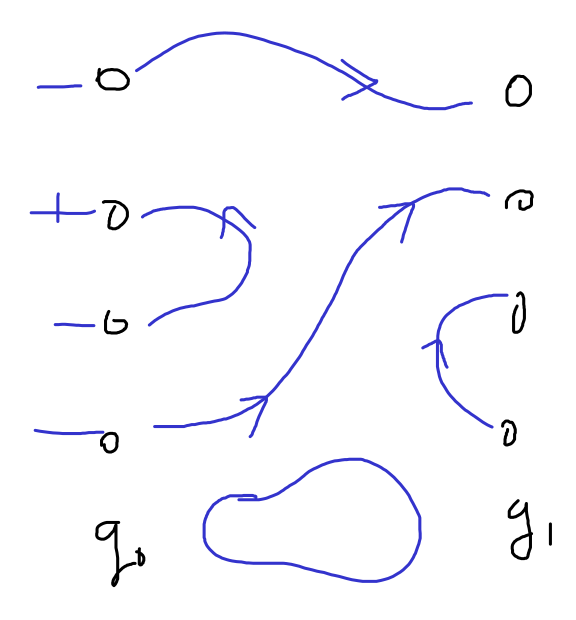
\includegraphics[width=0.3\linewidth]{figures/cobord.png}
\caption{The cobordism of moduli spaces.}
\label{cobord}
\end{figure}
We need $\mathcal P$ cut out transversely insides $[0,1] \times \mathcal B^*$, avoiding reducible solutions for all $g_t$. If  $b^+ > 1$, generic paths of metrics have no instantons. If $b^+  = 1$, we could encounter instantons in the path. This is the outcome:
\begin{itemize}
\setlength\itemsep{-.2em}
    \item If $b^+ X> 1$, we get $\mathrm{SW}_X \colon  \mathrm{Sp in}^c (X) \to \Z$, and  
        \[
        \mathrm{SW}_X(\mathfrak s) = 
        \begin{cases}
            \langle [\mathcal M_{\mathfrak s,g}], U ^{d(\mathfrak (s) / 2} \rangle & \text{if } d(\mathfrak s ) \in 2\Z,\\
            0 & \text{if } d(\mathfrak s) \text{ is odd.} 
        \end{cases}
        \] 
    \item If $b^+ X = 1$, $\mathrm{SW_X}$ depends on additional data.
    \item If $b^+X = 0$, we have no meaningful invariant.
\end{itemize}
We still need to talk about spin geometry and elliptic operators. Then we will get into Seiberg-Witten specific things like the compactness of the moduli space.



    \section{Elliptic operators and their symbols} 
Last time, for vector bundles $E \to M, F\to M$ vector bundles, we discussed the operator $\mathcal D \colon \Gamma(E) \to \Gamma(F)$. Then $\mathcal D$ is a 1st order operator iff $\mathcal D = L \circ j^1$. For every $f \in C ^{\infty}(M)$, we have the zeroth order $[\mathcal D,f]$, where $j^1 s \in \Gamma (J^1 E)$, $L \colon J^1 E  \to F$. So that's a fancy way of saying 1st order operators only depend on first order derivatives. The symbol \[
    \frac{\mathcal D(E,F)_1}{\mathcal D(E,F)_0} \xrightarrow[\sigma^1]{\cong } \Gamma (\Hom(T^*M\otimes E,F))
\] sends for $\xi_x \in T_x^* M$, $\sigma^1_{\mathcal D}(\xi_x) \colon E_x \to F_x$, where $\xi_x = (df)_x$, $\sigma^1_{\mathcal D}(\xi_x) = [\mathcal D, f]_x$. 
\begin{example}
    For the exterior derivative $d \colon \Omega^k_M \to \Omega^{k+1}_M$, we have $\sigma^1_d(\xi_x) \colon \Lambda^k_x  \to \Lambda^{k+1}_x$, since $[d,f] = df \wedge -$. So the symbol expresses that  $\xi_x $ is wedged with something else.
\end{example}
\begin{example}
    Consider the Dirac operator, with the trivial $\C^2$ bundle on $\C^3$. Then \[
    \mathcal D = \sigma_1 \frac{\partial }{\partial x_1}+ \sigma_2 \frac{\partial }{\partial x_2}+ \sigma_3 \frac{\partial }{\partial x_3}.
    \] The matrices are then given by \[
    \sigma_1 = 
    \begin{bmatrix}
        0 & 1 \\ 1 & 0
    \end{bmatrix},\quad 
    \sigma_2 = 
    \begin{bmatrix}
        i & 0 \\ 0 & -i 
    \end{bmatrix}, \quad
    \sigma_3 = 
    \begin{bmatrix}
        0 & 1 \\ -1 & 0 
    \end{bmatrix}
\] These are matrices chosen with the property that $\sigma_k ^2 = -I$, and $\sigma_j \sigma_k + \sigma_k \sigma_j  = 0$ if $j\neq k$. Then the symbol $\sigma^1_{\mathcal D}(dx_j ) = \sigma_j $.
\end{example}
The reason why this operator was introduced is because it squares to the geometer's Laplacian, or $\mathcal D^2 = -\sum \frac{\partial ^2}{\partial x_j ^2}$ (minus of the Laplacian). 
\begin{example}[Formal adjoints]
    Suppose we have the formal adjoints $E,F$ with hermitian metrics (for example bundles) or Euclidian if they're real. Let $g$ be a Riemannian metric on $M$. We have a first order operator $\mathcal D \colon \Gamma (E) \to \Gamma (F)$. Then a formal adjoint $\Gamma (E)\xleftarrow{\mathcal D^*} \Gamma (F)$ goes in the opposite direction, and is characterized by the fact that $\langle \mathcal D s, s' \rangle = \langle s, \mathcal D^* s' \rangle $ for  every $s \in \Gamma (E)$, $s' \in \Gamma (F)$. These are $L^2$ inner products, or $\int_M \left. (Ds,s') d\mu \right| _g$. Then if you think for a little bit, the following two expressions\[
            \langle t, [f,\mathcal D]s \rangle _{L^2(F)}= \langle [D^*,f]t,s \rangle _{L^2(E)}
    \] are the same. This tells us that the symbol of a formal adjoint applied to some cotangent vector is the same as the symbol of $\mathcal D$ applied to $\xi$, the taking the adjoint operator. In other words, \[
            \langle t, [f,\mathcal D]s \rangle _{L^2(F)}= \langle [D^*,f]t,s \rangle _{L^2(E)} \implies 
    \sigma^1 _{\mathcal D^*}(\xi) = -(\sigma^1_{\mathcal D}(\xi))^T.
    \] 
\end{example}
\begin{example}
    We can compute the symbol of $d^* \colon \Omega^k_M \to \Omega^{k-1}_M$; its symbol is simply given by $\sigma^1_{d^*}(\xi) = - \sigma^1_d(\xi)^* = -(\xi \wedge - )^*$. We just have to work out what the wedging operation is, which turns out to be pretty simple. Here we use the metric on forms induced by the Riemannian metric. So by a little bit of algebra, \[
        \sigma^1_{d^*}(\xi_x) = -i(\xi^{\flat}_x),\quad  \Lambda ^k _x \to \Lambda  ^{k-1}_x,\ \xi^{\flat}\in T_x M,\ \xi_x = g(\xi^{\flat}, -).
    \] We have not yet seen a formula for $d^*$, but in a sense this gives one.
\end{example}
\begin{definition}[]
    The first order operator $\mathcal D \in \mathcal D_1(E,F)$ is called \textbf{elliptic} if $\sigma^1_{\mathcal D}(\xi_x) \colon E_x \to F_x$ is a vector space isomorphism for all $x \in M$ and for all $(\xi_x \neq 0) \in T_x ^* M$.
\end{definition}
\begin{example}
    The Dirac operator $\mathcal D$ over $\R^3$ is elliptic since for $\sigma^1 _{\mathcal D}(\xi_x) \colon \C^2 \to \C^2$, we have $\sigma^1_{\mathcal D}(\xi)^2 = - |\xi|^2I$. This follows from the commutation relations between the matrices.
\end{example}
\begin{example}
    The exterior derivative takes $k$-forms to $k+1$-forms; this cannot be elliptic since the domain and codomain have different dimensions. But if we add it to the codimension and think of it as an operator on forms of arbitrary (mixed) degree, this has a chance of being elliptic. \[
    d \oplus d^* \colon \Omega^*_M \to \Omega^*_M
\] The symbol $\sigma^1 _{d\oplus d^*}(\xi_x) \colon \Lambda^*_x \to \Lambda^*_x$ is given by $\sigma^1(\xi) = (\xi \wedge -) - i(\xi^{\flat})$. It is not immediately obvious that this is an isomorphism, but you can check readily that $\sigma^1 _{d\oplus d^*}(\xi)^2 = -|\xi|^2\id$.
\end{example}
\begin{definition}[]
    A 1st order operator on $\mathcal \colon \Gamma (E) \to \Gamma (E)$ is called a \textbf{Dirac operator} if its symbol $\sigma^1 _{\mathcal D}(\xi)^2 = -|\xi|^2 \id$. 
\end{definition}
\begin{example}
    The \textbf{quantum Dirac operator}  on $\R^3$ is $d\oplus d^*$.
\end{example}
These examples are formally self adjoint, or $\mathcal D^* = \mathcal D$ (along with all operators of geometric interest). For a Dirac operator, $\sigma^1_{\mathcal D^*}=\sigma^1 _{\mathcal D}$, so $\mathcal D - \mathcal D^*$ is a 0th order operator. Some Dirac operators are $\Z/2$-graded, i.e. $E = E ^{\mathrm{ev}}\oplus E ^{\mathrm{odd}}$, where $\mathcal D \colon \Gamma(E ^{\mathrm{ev}}) \leftrightarrows \Gamma (E ^{\mathrm{odd}})  $. 
\begin{example}
    Let $(X^4, g)$ be a compact oriented Riemannian manifold, then \[
        d^* \oplus d^+ \colon \Omega^1_X \to \Omega^0_X \oplus \Omega^+_g,\quad \alpha  \mapsto  d^* \alpha  \oplus (d\alpha )^+.
    \] The symbol $\sigma^1 (\xi) \colon \Lambda^1_x \to \Lambda^0_x \oplus \Lambda^+_x$ is given by $\sigma^1(\xi) = -i(\xi ^{\flat})\oplus (\xi \wedge -)^+$. A quick check with an orthonormal basis on $\R^4$ shows that if $\xi\neq 0$, then $\sigma^1(\xi)$ is an isomorphism.
\end{example}
\subsection{Higher order operators and the Laplacian}
We have $n$th order operators $\mathcal D \colon \Gamma (E) \to \Gamma (F)$ vector spaces $\mathcal D_n (E,F)$, where $\mathcal D  \in \mathcal D_n (E,F) \iff [\mathcal D,f] \in \mathcal D_{n-1}(E,F)$ for every $f \in C ^{\infty}(M)$. Once again there is a story with jets; this is equivalent to saying that $\mathcal D = L \circ j^n $ for some $L \colon J^n E \to F$, where $J^n E$ is the bundle of $n$-jets of sections of $E$. Sections have the same $n$-jets at $x$ iff they have the same Taylor expansion to some order in the coordinates at $x$. There is an isomorphism $\sigma^n  \colon \frac{\mathcal D_n  (E,F)}{\mathcal D_m(E,F)}\to \Gamma \left(\mathrm{Sym}^n (T^*X)\otimes E,F\right)$, which means degree $n$ homogeneous polynomial functions on a vector space $T_x^* M$. As in the first order case, we can set up this isomorphism abstractly, or write it down in terms of commutators and functions. The formula is that for $\xi \in T_x^*M$, $\xi = (df)_*$ \[
        \sigma^n _{\mathcal D}(\underset{n}{\underbrace{\xi,\cdots ,\xi}} ) \colon E_x \to F_x,\quad \frac{1}{n!}\left[ \cdots \left[\left[\mathcal D,f\right],f\right] \cdots f\right]
    \] for $n$ copies of $f$, which is a linear map. This actually respects composition, that is, for $D_1 \in \mathcal D_m (E,F)$, $D_2 \in \mathcal D_n (F,G)$, their composite $D_2 \circ D_1 \in \mathcal D_{m+n}(E,G)$ with symbol given by $\sigma ^{m+1}_{D_2 \circ D_1}= \sigma^n _{D_2}\circ \mathcal D^m_{D_1}$.

    \section{Spinors, continued} 
We had $k$ a field, $(V,q)$ a quadratic $k$-space (vector space with a quadratic form on it). We build from that the Clifford algebra $\mathrm{Cl}(V,q) = \mathrm{Cl}^0 \oplus \mathrm{Cl}^1$, a $\Z/2$-graded associative unital $k$-algebra. If $\dim V = n$, then $\dim \mathrm{Cl}(V,q)= 2^n $. We began on spinors; a \textbf{spinor module} over some extension field $K$ is a $\Z/2$-graded $ K$-vector space $S = S^+ \oplus S^-$, with a representation $\rho \colon \mathrm{Cl}(V,q)\otimes K \to \mathrm{sEnd}(S)$, where  
\begin{equation*}
    \mathrm{Cl^0}\mapsto 
    \begin{bmatrix}
        *  & 0 \\ 0 & *
    \end{bmatrix},\quad
    \mathrm{Cl^0}\mapsto 
    \begin{bmatrix}
        0  & * \\ * & 0
    \end{bmatrix}
\end{equation*}
The spinor condition is that $\rho$ is actually an isomorphism of $\Z /2$-graded $K$-algebras.
\subsection{Construction of spinor modules}
Say $(V_k, q_k) \cong  (L \oplus L ^{\vee}, \mathrm{ev})$ with $\lambda\in L, \mu \in  L ^{\vee}$. Then $\mathrm{ev}(\lambda + \mu) = \mu(\lambda)$. If $q$ is non-degenerate of even rank and $K$ is algebraically closed ($\C$), fixing the rank all non-degenerate forms are isomorphic. Set $S = \Lambda ^* L ^{\vee}= \Lambda ^{\mathrm{ev}}L ^{\vee}\oplus \Lambda ^{\mathrm{odd}}L ^{\vee}$. When $\dim L = m$, we have \[
    \dim \mathrm{Cl}(V) = 2^{2m}= (2^m)^2,
\] so we want $\dim S = 2^m$ where $(S^+ = \Lambda ^{\mathrm{ev}}L ^{\vee})\oplus (S^- = \Lambda ^{\mathrm{odd}}L ^{\vee})$. We have that $\lambda \in  L$ leads to an ``annihilation operator'' $a(\lambda) = \iota_{\lambda} \colon \Lambda^k L ^{\vee} \to \Lambda^{k-1}L ^{\vee}$, and $\mu \in L ^{\vee}$ leads to a ``creation operator'' $c(\mu) = \mu \wedge - \colon \Lambda^k L ^{\vee} \to \Lambda^{k+1}L ^{\vee}$. The formula is that \[
\rho \colon L \oplus L ^{\vee} \to \mathrm{End}^1(S), \quad \rho (\lambda, \mu) = c(\mu) - a(\lambda).
\] One can check that the Clifford relations lead to an isomorphism $\rho \colon \mathrm{Cl}(L\oplus L^{\vee}) \to \mathrm{sEnd}(S)$. The easy case is where $\dim L = 1$. Then $L \oplus L ^{\vee}$ with $e \in L$ and $e^{\vee}\in  L ^{\vee}$ has basis $1, e, e ^{\vee}, ee ^{\vee} $, for the Clifford algebra, where $S = K \oplus L ^{\vee}$. Then \[
\rho(1)=
\begin{bmatrix}
    1 & 0 \\ 0 & 1
\end{bmatrix},\quad \rho(e) = 
\begin{bmatrix}
    0 & -1 \\ 0 & 0
\end{bmatrix},\quad \rho(e^{\vee})=
\begin{bmatrix}
    0 & 0 \\ 1 & 0 
\end{bmatrix},\quad \rho(ee ^v) = 
\begin{bmatrix}
    1 & 0 \\ 0 & -1
\end{bmatrix} 
\] which are isomorphic to  $\mathrm{sEnd}(S)$. In general, say $L = L_1\oplus \cdots \oplus L_m$ is a sum of lines, where $\mathrm{Cl}(L \oplus L ^{\vee}) \cong \widetilde{\bigotimes} _i \mathrm{Cl}(L_i \oplus L_i  ^{\vee})$, and $\Lambda^* L ^{\vee}\cong  \widetilde{\bigotimes} \Lambda^* L_i  ^{\vee} $, $\rho = \bigotimes \rho_i $ isomorphisms. For example, $\mathrm{Cl}(\R^4, |\cdot |^2)\otimes \C \xrightarrow{\cong } \mathrm{sEnd}(\Lambda^* \C^2)$, where $S^+ = \Lambda^0\oplus \Lambda^2, S = \Lambda^1$.

So far, we have the Clifford algebras and spinor modules. The next thing is the rigidity of spinors, and from this we get a projective (scalar ambiguity) action of $O(V)$ on $S$, or alternatively, on the Clifford algebra $\mathrm{Cl}(V,q)$ itself by invertible automorphisms. Differentiate to get a projective action of the Lie algebra of $O(V)$ on $\mathrm{Cl}(V,q)$ by inner derivations. This can be made concrete, or there is a formula. The spin groups allow us to resolve the scalar ambiguity, and in some sense that is what spin groups are for.

\subsection{Rigidity over $\C$}
The spinor module $S = S^+ \oplus S^- $ and its parity reversed version $\Pi S = S^- \oplus S^+$ are the only indecomposable representations. Every finite dimensional $\Z/2$-graded representation of $\mathrm{Cl}(V,q)$ is isomorphic to $S ^{\oplus r}\oplus \left( \Pi S \right) ^{\oplus s}$. Why? It is a standard fact from algebra is that the endormorphism of a vector space has  $S$ as its unique indecomposable (left) module. Since $\mathrm{Cl}(V,q) \cong  \mathrm{End}(S)$ (as an ungraded algebra), any module is a sum of copies of $S$. We need to account for the $\Z /2$-grading. The reason is the following; the even Clifford algebra $\mathrm{Cl}^0 (V,q) \cong  \mathrm{End}(S^+) \times \mathrm{End}(S^-)$, so its center $Z = \C \times \C$ reads off the decomposition of $S$ into $S^+ \oplus S^-$ by looking at extension spaces of central involutions. 
This corresponds to a central involution $\omega \in \mathrm{Cl}^0(V,q)$, where $\omega^2= 1$. Given a Clifford module $T$ which is indecomposable, we know that $T \cong  S$ in an ungraded sense. We read off the $+,-$ parts from the eigenspaces of $\omega$. Now $\omega = e_1 e_1^{\vee} \cdots e_m e_m^{\vee}$.

Now we come to the projective action. For $g \in O(V)$, this implies that $\mathrm{Cl}(g) \in \Aut  \mathrm{Cl}(V,q),  v_1 \cdots v_k \mapsto  gv_1 \cdots gv_k$. We have the action $\rho \colon \mathrm{Cl}(V,q) \to \mathrm{sEnd}(S)$, but we can also look at the representation $\rho \circ \mathrm{Cl}(g)$. By rigidity, these two representations are isomorphic, that is, there exists some $\overline{g} \colon S \to S$ so that $\rho \circ \mathrm{Cl}(g) \circ \overline{g} = \overline{g} \circ \mathrm{Cl}(g)$. We have that $\overline{g}$ is defined up to scalars, that is, we get a representation $\Theta \colon  g \to \Aut(S) / K ^{\times }  \mapsto \overline{g} $. The claim is that $[\rho \circ \mathrm{Cl}(g) ] \circ \overline{g} = \overline{g} \circ \rho$.



    %add and swap as necessary
\end{document}
